\documentclass{article}
\usepackage[parfill]{parskip}
\usepackage[utf8]{inputenc}
\usepackage{amsmath}
\usepackage{amsthm} % for proofs
\usepackage{amssymb}
\usepackage{graphicx}
\usepackage{bm}
\usepackage[toc,page]{appendix}
\graphicspath{ {./images} }

\title{Notes on statistical learning}
\author{Dávid Iván}

\begin{document}

\maketitle

\tableofcontents

\newpage
\section{Introduction}
\section{Overview of Supervised Learning}
\subsection{Linear models and least squares}

On page 12 we have that the residual sum of squares:

\begin{equation}
    \text{RSS}(\beta) = \sum_{i=1}^{N}(y_i-x_i^T\beta)^2 = (\textbf{y} - \textbf{X}\beta)^T(\textbf{y} - \textbf{X}\beta)
\end{equation}

How can we differentiate with respect to $\beta$?

\begin{equation}
    \text{RSS}(\beta) = \textbf{y}^T\textbf{y} - \textbf{y}^T\textbf{X}\beta - \beta^T \textbf{X}^T \textbf{y} + \beta^T \textbf{X}^T \textbf{X} \beta
\end{equation}

Using (\ref{eq:da_dx}, \ref{eq:dA_dx}), we can differentiate RSS:

\begin{equation}
    \frac{d}{d\beta} \text{RSS}(\beta) = 0 - (\textbf{y}^T \textbf{X})^T - \textbf{X}^T\textbf{y} + (\textbf{X}^T\textbf{X} + (\textbf{X}^T\textbf{X})^T)\beta
\end{equation}

\begin{equation}
    \frac{d}{d\beta} \text{RSS}(\beta) =  -2 \textbf{X}^T\textbf{y} + 2\textbf{X}^T\textbf{X}\beta
\end{equation}

Setting this to zero we get the normal equations:

\begin{equation}
    \textbf{X}^T\textbf{y} = \textbf{X}^T\textbf{X}\beta
\end{equation}

\newpage
\subsection{Statistical decision theory} \label{linear_fit}

On page 19 we have that

\begin{equation} \label{eq:2_beta}
    \beta = [E(XX^T)]^{-1}E(XY)
\end{equation}

but how exactly do we get this equation? In general, we have the expected prediction error:
\begin{equation}
    \text{EPE}(f) = E(Y-f(X))^2
\end{equation}

And we have that the prediction function is linear:
\begin{equation}
    f(X) = X^T\beta
\end{equation}

We seek a $\beta$ for minimizing the expected prediction error. $X$ and $Y$ are random variables, $X$ being a vector, $Y$ being a scalar. 
\begin{equation}
    \begin{split}
        \frac{d}{d\beta}\text{EPE} = \frac{d}{d\beta} \text{E}((Y-X^T\beta)^2) = \text{E}\left( \frac{d}{d\beta} (Y-X^T\beta)^2\right)\\
        =\text{E} \left( 2(Y - X^T\beta)\cdot (-X) \right) = -2 \text{E} (YX) + 2 \text{E} (X(X^T\beta))\\
         = -2 \text{E} (YX) + 2 \text{E} ((XX^T)\beta) = -2 \text{E} (YX) + 2 (\text{E} (XX^T))\beta
    \end{split}
\end{equation}

We used the fact that the expected value is linear, and that $\beta$ is not random, so we could factor out from the expected value. Setting this to zero we have that:

\begin{equation}
    \text{E} (YX) = \text{E} (XX^T)\beta
\end{equation}

which yields

\begin{equation}
    \hat{\beta} = [\text{E} (XX^T)]^{-1} \text{E} (YX)
\end{equation}

\subsubsection{application. Simple linear fit.}

Let's see an application for this equation. Let $X=\begin{bmatrix}x\\ 1\end{bmatrix}$, $\beta = \begin{bmatrix}a\\b\end{bmatrix}$.

Now $f(x) = a\cdot x + b$

\begin{equation}
    XY = \begin{bmatrix}x\cdot y \\ y\end{bmatrix}
\end{equation}

\begin{equation}
    XX^T = \begin{bmatrix} x^2 & x \\ x & 1 \end{bmatrix}
\end{equation}

If we have $N$ datapoints $\{(x_1, y_1), (x_2, y_2), ... (x_N, y_N)\}$, we can approximate the expectation values.

\begin{equation}
    \text{E}(XY) \approx \frac 1N \begin{bmatrix}\sum_i x_i\cdot y_i \\ \Sigma_i y_i\end{bmatrix}
\end{equation}

\begin{equation}
    \text{E}(XX^T) \approx \frac 1N \begin{bmatrix} \sum_i x^2_i & \Sigma_i x_i \\ \Sigma_i x_i & N \end{bmatrix}
\end{equation}

Let's denote the followings:

\begin{equation}
    \alpha_X = \sum_i x_i
\end{equation}

\begin{equation}
    \alpha_Y = \sum_i y_i
\end{equation}

\begin{equation}
    \alpha_{XY} = \sum_i x_i y_i
\end{equation}

\begin{equation}
    \alpha_{X^2} = \sum_i x^2_i
\end{equation}

With these notations:

\begin{equation}
    \text{E}(XY) \approx \frac 1N \begin{bmatrix} \alpha_{XY} \\ \alpha_Y \end{bmatrix}
\end{equation}

\begin{equation}
    \text{E}(XX^T) \approx \frac 1N \begin{bmatrix} \alpha_{X^2} & \alpha_X \\ \alpha_X & N \end{bmatrix}
\end{equation}

Inverting $\text{E}(XX^T)$:

\begin{equation}
    [\text{E}(XX^T)]^{-1} \approx \frac{N}{N\alpha_{X^2} - \alpha^2_X} \begin{bmatrix} N & -\alpha_X \\ -\alpha_X & \alpha_{X^2} \end{bmatrix}
\end{equation}

Plug these in to the equation:

\begin{equation}
    \hat{\beta} = [\text{E} (XX^T)]^{-1} \text{E} (YX)
\end{equation}

\begin{equation}
    \hat{\beta} \approx \frac{N}{N\alpha_{X^2} - \alpha^2_X} \begin{bmatrix} N & -\alpha_X \\ -\alpha_X & \alpha_{X^2} \end{bmatrix} \frac 1N \begin{bmatrix} \alpha_{XY} \\ \alpha_Y \end{bmatrix}
\end{equation}

\begin{equation}
    \hat{\beta} \approx \frac{1}{N\alpha_{X^2} - \alpha^2_X} \begin{bmatrix} N \alpha_{XY} -\alpha_X \alpha_Y \\ \alpha_{X^2} \alpha_Y - \alpha_X \alpha_{XY} \end{bmatrix}
\end{equation}


From here we can get $\hat{a}$ and $\hat{b}$, since $\hat{\beta} = \begin{bmatrix} \hat{a} \\ \hat{b} \end{bmatrix}$

\newpage
\subsection{$\text{E}|Y - c|$ and the median}

On page 20, it asks the question "What happens if we replace the $L_2$ loss function with the $L_1: \text{E}|Y-f(X)|$ ?" Let's investigate this question.

\subsubsection{discrete case}

We can get rid of the conditional $X=x$, and just ask the question: What $c$ will minimize $\text{E}|Y-c|$? Denote this function with $g$,  so $g(c) = \text{E}|Y-c|$. Let's look at two examples.

Example 1. The random variable $Y$ takes 4 possible values with probabilities $\frac 17$, $\frac 17$, $\frac 37$, $\frac 27$. The figure below shows the probability mass funciton.

\begin{figure}[ht]
 \centering
  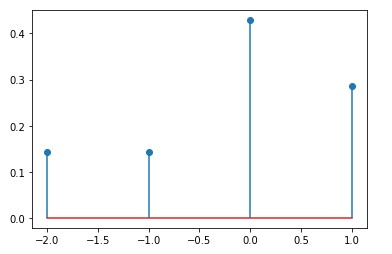
\includegraphics[width=200pt]{images/rnd1}
 \caption{probability mass function of the first example random variable.}
\end{figure}

\begin{figure}[ht]
 \centering
  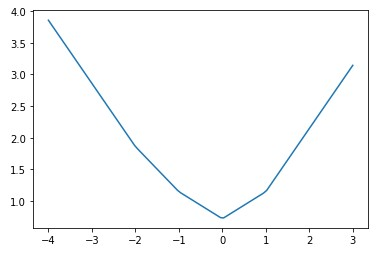
\includegraphics[width=200pt]{images/rnd_func1}
 \caption{$g(c)$ function. The horizontal axis is $c$.}
\end{figure}

Example 2. The random variable $Y$ takes 4 possible values with probabilities 0.1, 0.4, 0.3, 0.2. The figure below shows the probability mass funciton.

\begin{figure}[ht]
 \centering
  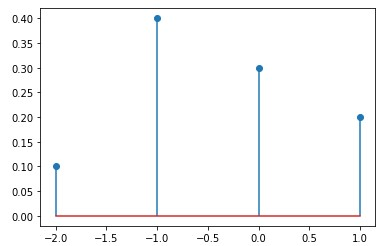
\includegraphics[width=200pt]{images/rnd2}
 \caption{probability mass function of the second example random variable.}
\end{figure}

\begin{figure}[ht]
 \centering
  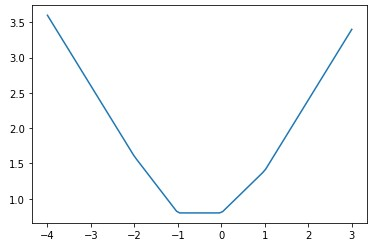
\includegraphics[width=200pt]{images/rnd_func2}
 \caption{$g(c)$ function. The horizontal axis is $c$.}
\end{figure}

We can see that $g(c)$ is a piecewise linear function, and it has minimum, which is a point or a line segment. Let's say we have $Y$ discrete random variable that takes values from $S=\{x_1, x_2, \dots x_n\}$. The values are ordered: $x_1 <  x_2 < ... < x_n$. $Y$ takes these values with corresponding probabilities $p_1$, $p_2$, ..., $p_n$.

Let's calculate the equation of the piecewise linear function. Denote the interval $I_k$ such that $x\in I_k$ if and only if $k$ values from $S$ are smaller than $x$. So $I_0 = (-\infty, x_1]$, $I_1 = [x_1, x_2]$, ..., $I_n = [x_n, \inf)$.

\begin{equation}
    g(c) = \text{E} |Y-c| = \Sigma_{i=1}^{n}p_i \cdot |x_i - c|
\end{equation}

If $c \in I_k$, then

\begin{equation}
    g(c) = \text{E} |Y-c| = \Sigma_{i=1}^{k}p_i \cdot (c - x_i) + \Sigma_{i=k+1}^{n}p_i \cdot (x_i - c)
\end{equation}

\begin{equation}
    g(c) = c\cdot (\Sigma_{i=1}^{k}p_i - \Sigma_{i=k+1}^{n}p_i) + (\Sigma_{i=k+1}^{n}p_i x_i - \Sigma_{i=1}^{k}p_i x_i)
\end{equation}

First we can show that this function is continuous. On one hand ($c\in I_k = [x_k, x_k+1]$):

\begin{equation}
    g_1 = g(x_k) = x_k\cdot (\Sigma_{i=1}^{k}p_i - \Sigma_{i=k+1}^{n}p_i) + (\Sigma_{i=k+1}^{n}p_i x_i - \Sigma_{i=1}^{k}p_i x_i)
\end{equation}

On the other hand we have ($c\in I_{k-1} = [x_{k-1}, x_k]$):

\begin{equation}
    g_2 = g(x_k) = x_k\cdot (\Sigma_{i=1}^{k-1}p_i - \Sigma_{i=k}^{n}p_i) + (\Sigma_{i=k}^{n}p_i x_i - \Sigma_{i=1}^{k-1}p_i x_i)
\end{equation}

\begin{equation}
    g_1 - g_2 = x_k \cdot (p_k + p_k) - p_k x_k - p_k x_k = 0
\end{equation}

Now that we showed that this function is continuous, let's find it's minimum. Since it is piecewise linear, its derivative is piecewise constant. Denote the derivative of $g$ on the interval $I_k$ with $g'(I_k)$.

\begin{equation}
    \begin{split}
        g'(I_k) = -1\\
        g'(I_1)= -1+2p_1\\
        g'(I_2)= -1+2p_1+2p_2\\
        \dots\\
        g'(I_n)= -1+2p_1+...+2p_n=1
    \end{split}
\end{equation}

So the derivative is increasing from $-1$ to $+1$. We can distinguish two possibilities. First, assume that the derivative is never zero. In this case, we have a $k$ where $g'(I_{k-1}) < 0$ but $g'(I_k) > 0$, so the minimum is at $x_k$, the median. The second case is where there is an interval where the derivative is zero. In this case the whole interval is minimum, again, the median.

\subsubsection{continuous case}

Let's have the following function:

\begin{equation}
    f(x) = \int_{a}^{x}g(x,t)dt
\end{equation}

I state without proof that the derivative of this function is as follows:

\begin{equation}
f'(x) = \int_{a}^{x} \frac{\partial g(x,t)}{\partial x} dt + g(x, x)
\end{equation}

Now we have that

\begin{equation}
    g(c) = \text{E}(|Y-c| | X=x) = \int_{-\infty}^{c}(c-y)f_{Y|X}(y|x)dy + \int_{c}^{\infty}(y-c)f_{Y|X}(y|x)dy
\end{equation}

\begin{equation}
    g'(c) = \int_{-\infty}^{c}f_{Y|X}(y|x)dy + \int_{\infty}^{c}f_{Y|X}(y|x)dy
\end{equation}

Setting this to zero, we get that

\begin{equation}
    \int_{-\infty}^{c}f_{Y|X}(y|x)dy = \int_{c}^{\infty}f_{Y|X}(y|x)dy
\end{equation}

\begin{equation}
    P(Y<c \mid X=x) = P(Y>c \mid X=x)
\end{equation}

Again, this means the minimum is at the median.


\newpage
\subsection{Local methods in high dimensions}

\subsubsection{deriving the prediction formula}

On page 24 we see an example of a linear data with noise. At first I was confused how it gets $\hat{y}_0 = x_0^T \beta + \sum_{i=1}^N l_i(x_0)\epsilon_i$, where $l_i(x_0)$ is the $i$th element of $\textbf{X}(\textbf{X}^T\textbf{X})^{-1}x_0$

In this example we make $N$ experiments, storing the $X_i$ values in the rows of $\textbf{X}$, and we have also $\epsilon_i$ (elements of $\vec{\epsilon}$) and $Y_i = X_i^T\beta + \epsilon_i$ for some fixed $\beta$. For approximating $\beta$, we use the result:

\begin{equation}
    \beta = [\text{E} (XX^T)]^{-1} \text{E} (YX)
\end{equation}

in this case it will be an approximation, since we have noise ($\epsilon$).

Calculate first $\text{E} (YX)$:

\begin{equation}
    \text{E} (YX) = \text{E} ((X^T\beta + \epsilon)X) = \text{E} (XX^T)\beta + \text{E} (\epsilon X)
\end{equation}

Substitute this into the approximation of $\beta$:

\begin{equation}
    \begin{split}
        \hat{\beta} = [\text{E} (XX^T)]^{-1} \text{E} (YX)\\
        = [\text{E} (XX^T)]^{-1} (\text{E} (XX^T)\beta + \text{E} (\epsilon X))\\
        = \beta + [\text{E} (XX^T)]^{-1} \text{E} (\epsilon X)
    \end{split}
\end{equation}

We do not know of course the exact expectation values, but we have $N$ data samples (training data). So how could we approximate the expectation values? Use the averages:

\begin{equation}
    \text{E}(\epsilon X)_i \approx \frac{1}{N} \sum_{k=1}^N \textbf{X}_{ki} \epsilon_k \to \text{E} (\epsilon X) \approx \frac{1}{N} \textbf{X}^T \vec{\epsilon}
\end{equation}

similarly,

\begin{equation}
    [\text{E} (XX^T)]^{-1} \approx N \cdot (\textbf{X}^T \textbf{X})^{-1}
\end{equation}

putting these all together, we have:

\begin{equation}
    \hat{y}_0 = x_0^T \hat{\beta} = x_0^T \beta + x_0^T (\textbf{X}^T\textbf{X})^{-1} \textbf{X}^T \vec{\epsilon} = x_0^T \beta + \vec{\epsilon}^T \cdot \textbf{X} (\textbf{X}^T \textbf{X})^{-1} x_0
\end{equation}

and this is the formula that was to be explained.


\subsubsection{equation (2.47) on page 37}

\begin{equation}
  \begin{split}
    \text{EPE}_k(x_0) = \text{E}\left((Y - \hat{f}_k(x_0))^2 | X=x_0\right)\\
    = \text{E}\left((f(x_0) + \epsilon_0 - \hat{f}_k(x_0))^2\right)
  \end{split}
\end{equation}

The data points are fixed: {$x_1, x_2, \dots, x_N$}. Denote the closest data point to $x_0$ as $x_{(1)}$, the second closest $x_{(2)}$, etc. With this notation, the nearest neighbor estimate for $f(x_0)$:

\begin{equation}
    \hat{f}_k(x_0) = \frac 1k \sum_{l=1}^{k}(f(x_{(l)}) + \epsilon_l)
\end{equation}

In this equation, $f(x_{(l)})$ is fixed, and epsilons are iid random variables.

\begin{equation}
  \begin{split}
    \text{EPE}_k(x_0) = \text{E}\left( \left(f(x_0) + \epsilon_0 - \frac 1k \sum_{l=1}^{k}(f(x_{(l)}) + \epsilon_l)\right)^2\right)\\
    = \text{E}\left( \left[ \left( f(x_0) - \frac 1k \sum_{l=1}^{k}f(x_{(l)})\right) + \left( \epsilon_0 - \frac 1k \sum_{l=1}^{k}\epsilon_l \right) \right]^2 \right)\\
    = \text{E} \left([\hat{F} + \hat{E}]^2\right) = \text{E} \left(\hat{F}^2 + 2\cdot \hat{F} \hat{E} + \hat{E}^2\right) = \hat{F}^2 + 2\hat{F}\cdot\text{E}(\hat{E}) + \text{E}(\hat{E}^2)
  \end{split}
\end{equation}

where $\hat{F}$ is nonrandom, and $\hat{E}$ is random:

\begin{equation}
  \begin{split}
    \hat{F} \equiv f(x_0) - \frac 1k \sum_{l=1}^{k}f(x_{(l)}),\\
    \hat{E} \equiv \epsilon_0 - \frac 1k \sum_{l=1}^{k}\epsilon_l
  \end{split}
\end{equation}

Let's calculate the expectation of $\hat{E}$:

\begin{equation}
    \text{E} (\hat{E}) = \text{E} \left( \epsilon_0 - \frac 1k \sum_{l=1}^{k}\epsilon_l \right) = \text{E} (\epsilon_0) - \frac 1k \sum_{l=1}^{k}\text{E} (\epsilon_l) = 0 - \frac 1k \sum_{l=1}^{k}0 = 0
\end{equation}

The expectation of $\hat{E}^2$:

\begin{equation}
    \text{E} (\hat{E}^2) = \text{E} \left( \epsilon_0 - \frac 1k \sum_{l=1}^{k}\epsilon_l \right)^2 = \text{E} \left( \epsilon_0^2 + \sum_{l=1}^{k}\frac{\epsilon_l^2}{k^2} + CrossProducts \right)
\end{equation}

The expectation of the cross products are zero, since epsilons are independent, so $\text{E}(\epsilon_i \epsilon_j) = \text{E} \epsilon_i \cdot \text{E} \epsilon_j = 0\cdot 0 = 0$

\begin{equation}
  \begin{split}
    \text{E} (\hat{E}^2) = \text{E} \left( \epsilon_0^2 + \sum_{l=1}^{k}\frac{\epsilon_l^2}{k^2} \right) = \text{E} \epsilon_0^2 + \sum_{l=1}^{k}\frac{\text{E}\epsilon_l^2}{k^2}\\
    = \sigma^2 + \sum_{l=1}^{k}\frac{\sigma^2}{k^2} = \sigma^2 + \frac{\sigma^2}{k}
  \end{split}
\end{equation}

We used the fact that the error has zero mean, so the variance is $\sigma^2 = \text{Var}(\epsilon) = \text{E}(\epsilon^2) - (\text{E}\epsilon)^2 = \text{E}(\epsilon^2)$. So the final form is:

\begin{equation}
  \begin{split}
    \text{E}_k(x_0) = \hat{F}^2 + 2\hat{F}\cdot\text{E}(\hat{E}) + \text{E}(\hat{E}^2) = \hat{F}^2 + \text{E}(\hat{E}^2)\\
    = \left( f(x_0) - \frac 1k \sum_{l=1}^{k}f(x_{(l)}) \right)^2 + \sigma^2 + \frac{\sigma^2}{k}
  \end{split}
\end{equation}

\subsection{Solutions for the Exercises of chapter 2}

\subsubsection{Ex. 2.2}

We have $X \in \mathbb{R}^p$ continuous and $G$ discrete random variables. Assume we have $K$ classes. Each class has its own distribution, let's say that class $g$ has a pdf $f_{g}(x)$ ($x \in \mathbb{R}^p$). When generating points, we first choose a class with associated probabilities $p_1, p_2, \dots, p_K$ ($\sum p_i = 1$). When we have chosen the class, we generate a point with the appropriate distribution.

The Bayes classifier classifies each point $x$ to the most probable class. So let's calculate the probability of class $g$, given the point. It should be noted that when I write $\text{P}(x)$, I mean "the probability that the chosen point is in the infinitesimal neighborhood of $x$". So I should write $\text{P}(X \in b_{dx}(x))$, i.e., the probability that $X$ is in the $dx$-volume ball around $x$. If the pdf was $f(x)$, this probability is $f(x)dx$. But instead, I'll write $\text{P}(x) = f(x)$. Likewise, when I write $\text{P}(g)$, I mean $\text{P}(G=g)$.

\begin{equation}
    \text{P}(g|x) = \frac{\text{P}(g \cap x)}{\text{P}(x)} = \frac{\text{P}(g \cap x)}{\text{P}(x)} = \frac{\text{P}(x | g) \text{P}(g)}{\sum_{g'}\text{P}(x|g') \text{P}(g')}
\end{equation}

The denominator is a normalizing constant, so the chosen class, for which $\text{P}(g|x)$ is maximum:

\begin{equation}
    \hat{g}(x) = max_{g} \text{P} (x|g) \text{P}(g)
\end{equation}

\subsubsection{Ex. 2.3}

Given a unit ball in $p$-dimension. We sample $N$ data points from it uniformly. Let $X$ be the distance from the origin. The pdf must be proportional to $x^{p-1}$, and integrating it from 0 to 1 gives 1, thus the pdf:

\begin{equation}
    f(x) = p\cdot x^{p-1}
\end{equation}

The probability that a random sample is at least $x$ distant from the origin is:

\begin{equation}
    \text{P}(X > x) = \int_{x}^{1} f(x)dx = 1 - x^p
\end{equation}

The probability that all $N$ sample points are further from origin as $x$:

\begin{equation}
    \text{P}(X_1 > x \cap X_2 > x \cap \dots \cap X_N > x) = \left( 1 - x^p \right)^N
\end{equation}

We seek and $x$ for that this probability is a half (that will give us the median):

\begin{equation}
  \begin{split}
    \left( 1 - x^p \right)^N = \frac 12\\
    1 - x^p = \left(\frac 12\right)^{1/N}\\
    \left[1 - \left(\frac 12\right)^{1/N}\right]^{1/p} = x
  \end{split}
\end{equation}


\subsubsection{Ex. 2.4}

If we choose $a$ as the first unit base vector ($a=[1,0,0,\dots,0]^T$), then $a^T \cdot x_i$ is the first coordinate of $x_i$. It is by definition (standard) normally distributed. Since the distribution is spherically symmetric, we can choose any direction $a$, $a^T \cdot x_i$ remains standard normal.

I created an experiment on this. Created 1000 sample points in $p$ dimension, and rotated them into the first 2 dimension, so that we can visualize the distances. On the first image below we can see that the points get further and further away from the origin as the dimension increases.

\begin{figure}[ht]
 \centering
  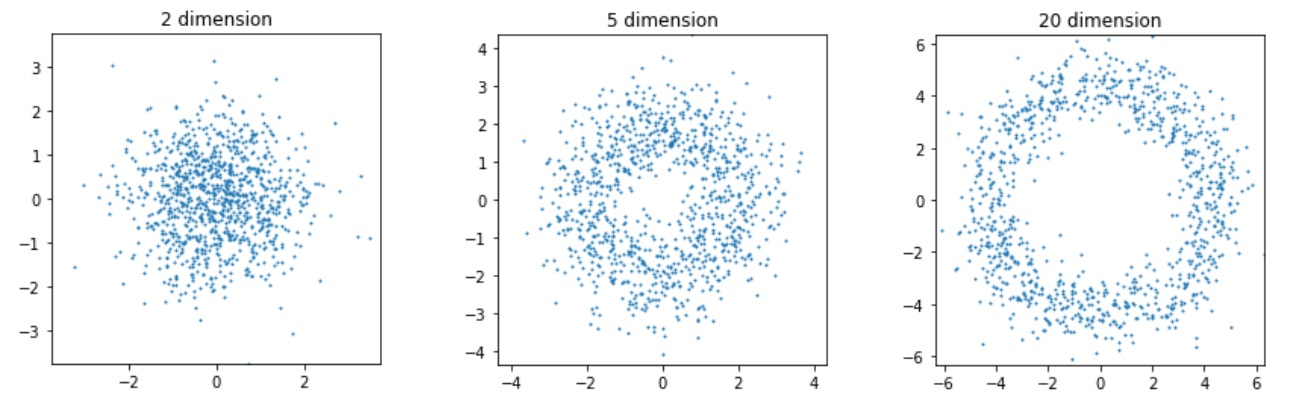
\includegraphics[width=200pt]{images/ex2_2_origin.jpg}
 \caption{The sample points get further from the origin as we increase the dimension.}
\end{figure}

But this doesn't mean the points are close to each other. In the following experiment I took the random sample points, chose one of them and set it as the new origin. We can see that still the points are far from a random sample point as we increase the dimension.

\begin{figure}[ht]
 \centering
  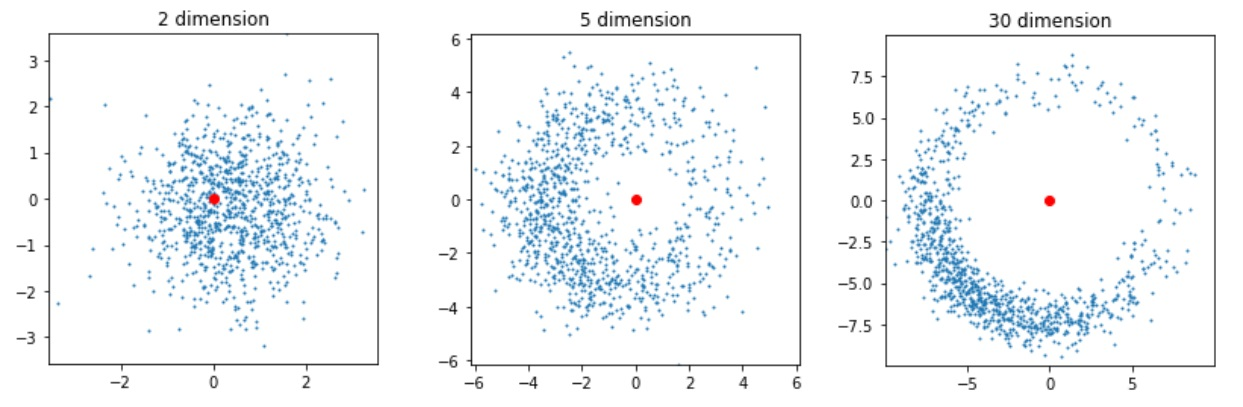
\includegraphics[width=200pt]{images/ex_2_2_sample.jpg}
 \caption{The points get further and further from each other (red dot is a randomly selected sample point) as we increase the dimension.}
\end{figure}

\subsubsection{Ex. 2.5}

\paragraph{equation (2.27) on page 26}

I won't use indices at the expectation sign, it always confuses me. So this is the expected prediction error:

\begin{equation}
    \text{EPE}(x_0) = \text{E}(y_0 - \hat{y}_0)^{2}
\end{equation}

Recall, that $y_0 = x_0^T \beta + \epsilon$ is a random variable, since $\epsilon \sim N(0,\sigma^2)$. This is the label (the ground truth) for $x_0$. The prediction that we make for $x_0$ is $\hat{y_0} = x_0^T \beta + \vec{\epsilon}^T \cdot \textbf{X} (\textbf{X}^T \textbf{X})^{-1} x_0$. $x_0$ is a $p$-vector, $\beta$ is a $p$-vector, $\vec{\epsilon}$ is an $n$-vector, and $\mathbf{X}$ is a $n$ by $p$ matrix (each row is a training sample vector). $\hat{y}_0 = x_0^T \beta + \vec{\epsilon}^T \cdot \textbf{Z}^T x_0$. Here I introduced the $p$ by $n$ matrix $\textbf{Z}$:

\begin{equation}
    \textbf{Z} \equiv (\textbf{X}^T \textbf{X})^{-1} \textbf{X}^T
\end{equation}

In the expression of $\hat{y}_0$, $\vec{\epsilon}$ and $\textbf{Z}$ are the only random variables. The elements of $\vec{\epsilon}$ are iid RVs. $\vec{\epsilon}$ and $\textbf{Z}$ are independent. Let's calculate the expectation values of $y_0$ and $\hat{y}_0$:

\begin{equation}
    \text{E}(y_0) = \text{E} (x_0^T \beta + \epsilon) = x_0 ^ T \beta
\end{equation}

\begin{flalign}
  \begin{aligned}
    \text{E}(\hat{y}_0) =& \text{E} (x_0^T \beta + \vec{\epsilon}^T \cdot \textbf{Z}^T x_0)\\
    =& x_0^T \beta + \text{E}(\vec{\epsilon}^T \cdot \textbf{Z}^T x_0) \\
    =& x_0^T \beta + \text{E}(\vec{\epsilon}^T) \text{E} (\textbf{Z}^T x_0) \\
    =& x_0^T \beta + \vec{0}^T \cdot \text{E} (\textbf{Z}^T x_0) \\
    =& x_0^T \beta
  \end{aligned}
\end{flalign}

Here I used that $\vec{\epsilon}$ and $\textbf{Z}$ are independent, so the expectation value of their product is the product of their expectations. For simplicity, denote $\mu \equiv \text{E}(y_0) = \text{E}(\hat{y}_0) = x_0^T \beta$. The expected prediction error:

\begin{flalign}
  \begin{aligned}
    \text{EPE}(x_0) =& \text{E} (y_0 - \mu + \mu - \hat{y}_0)^2 \\
    =& \text{E} (y_0 - \mu) ^ 2 - 2 \cdot \text{E} ((y_0 - \mu)(\hat{y}_0 - \mu)) + \text{E} (\hat{y}_0 - \mu)^2\\
    =& \text{E} (y_0 - \mu) ^ 2 + 0 + \text{E} (\hat{y}_0 - \mu) ^ 2\\
    =& \text{Var}(y_0) + \text{Var}(\hat{y}_0)
  \end{aligned}
\end{flalign}

Note that $y_0$ and $\hat{y}_0$ are independent. The epsilon in $y_0$ is a scalar and is nothing to do with the vector epsilon in $\hat{y}_0$. This is why $\text{E} ((y_0 - \mu)(\hat{y}_0 - \mu))$ is zero. Now let's derive the variances:

\begin{equation}
    \text{Var}(y_0) = \text{Var}(\mu + \epsilon) = \text{Var}(\epsilon) = \sigma ^2
\end{equation}

Furthermore, we can write $\text{Cov}(X,X) = \text{E} ((X-\text{E}X)\cdot (X-\text{E}X)^T) = \text{E}(X\cdot X^T) - (\text{E}X) (\text{E}X^T)$. Let's apply (\ref{eq:vector_mul_variance}) and (\ref{eq:covariance_formulae}) to derive the variance of $\hat{y}_0$:

\begin{flalign} \label{eq:1}
  \begin{aligned}
    \text{Var}(\hat{y}_0) =& \text{Var}(\mu + x_0^T \cdot \textbf{Z} \cdot \vec{\epsilon}) = \text{Var} (x_0^T \cdot \textbf{Z} \cdot \vec{\epsilon})\\
     =& x_0^T \cdot \text{Cov}(\textbf{Z} \cdot \vec{\epsilon}, \textbf{Z} \cdot \vec{\epsilon}) \cdot x_0\\
     =& x_0^T \cdot \left( \text{E}(\textbf{Z} \vec{\epsilon} \cdot \vec{\epsilon}^T \textbf{Z}^T) - \text{E}(\textbf{Z}\vec{\epsilon}) \cdot \text{E} (\vec{\epsilon}^T \textbf{Z}^T) \right) \cdot x_0\\
     =& x_0^T \cdot \text{E}(\textbf{Z} \vec{\epsilon} \cdot \vec{\epsilon}^T \textbf{Z}^T)  \cdot x_0
  \end{aligned}
\end{flalign}

Here we used the fact that $\textbf{Z}$ and $\vec{\epsilon}$ are independent, so $\text{E}(\textbf{Z} \vec{\epsilon}) = \text{E}\textbf{Z} \cdot \text{E} \vec{\epsilon} = \text{E}\textbf{Z} \cdot \vec{0} = \vec{0}$, and $\vec{0} \cdot \vec{0}^T = \textbf{0}$, zero matrix.

\begin{equation}
  \begin{split}
    \left( \textbf{Z} \vec{\epsilon} \cdot \vec{\epsilon}^T \textbf{Z}^T \right)_{i,j} = \sum_{k,l} (\textbf{Z})_{i,k} \cdot (\vec{\epsilon} \vec{\epsilon}^T)_{k,l} \cdot (\textbf{Z}^T)_{l,j}\\
    \to \text{E} \left( \textbf{Z} \vec{\epsilon} \cdot \vec{\epsilon}^T \textbf{Z}^T \right)_{i,j} = \sum_{k,l} \text{E} \left( Z_{i,k} \cdot \epsilon_k \cdot \epsilon_l \cdot Z_{j,l} \right)\\
    = \sum_{k,l} \text{E} \left( Z_{i,k} \cdot Z_{j,l} \right) \cdot \text{E} \left( \epsilon_k \cdot \epsilon_l \right) = \sum_{k,l} \text{E} \left( Z_{i,k} \cdot Z_{j,l} \right) \cdot \sigma^2 \delta_{k,l}\\
    = \sigma^2 \cdot \sum_{k} \text{E} \left( Z_{i,k} \cdot Z_{j,k} \right) = \sigma^2 \cdot \text{E} \sum_{k} \left( Z_{i,k} \cdot Z_{j,k} \right) = \sigma^2 \cdot \text{E} (\textbf{Z} \textbf{Z}^T)_{i,j}\\
    \to \text{E}(\textbf{Z} \vec{\epsilon} \cdot \vec{\epsilon}^T \textbf{Z}^T) = \sigma^2 \cdot \text{E} (\textbf{Z} \textbf{Z}^T)
  \end{split}
\end{equation}

Substituting this into (\ref{eq:1}):

\begin{equation}
    \text{Var}(\hat{y}_0) = x_0^T \cdot \sigma^2 \text{E} (\textbf{Z} \textbf{Z}^T) \cdot x_0
\end{equation}

\begin{equation}
    \text{E}(\textbf{Z} \textbf{Z}^T) = \text{E} \left( (\textbf{X}^T \textbf{X})^{-1} \textbf{X}^T \textbf{X} (\textbf{X}^T \textbf{X})^{-1} \right) = \text{E} \left( (\textbf{X}^T \textbf{X})^{-1} \right)
\end{equation}

Putting it all together:

\begin{equation}
    \text{EPE}(x_0) = \text{Var} (y_0) + \text{Var} (\hat{y}_0) = \sigma^2 + \sigma^2 \cdot x_0^T \cdot \text{E} \left( (\textbf{X}^T \textbf{X})^{-1} \right) \cdot x_0
\end{equation}

And this is what we wanted to derive.

\paragraph{equation (2.28) on page 26}

\begin{equation}
    \text{E} \left( x^T_0 \text{Cov}(X)^{-1}x_0 \right) = \text{E} \sum_{i,j} x_{0,i} \text{Cov}(X)^{-1}_{i,j} x_{0,j}
\end{equation}

Assuming that $x_0 \sim X$, i.e., $x_0$ (the test point) has the same distribution as $X$ (the training data), and the expectation of it is the zero vector, $\text{Cov}(x_0) = \text{Cov}(X) = \text{E} (x_0 x^T_0)$.

\begin{equation}
  \begin{split}
    \text{E} \sum_{i,j} x_{0,i} \text{Cov}(X)^{-1}_{i,j} x_{0,j} = \text{E} \sum_{i,j} \text{Cov}(X)^{-1}_{i,j} \text{Cov}(x_0)_{i,j}\\
    = \text{E} \sum_{i,j} \text{Cov}(X)^{-1}_{i,j} \text{Cov}(X)_{i,j} = \text{E} \sum_{i} \left( \sum_{j} \text{Cov}(X)^{-1}_{i,j} \text{Cov}(X)_{j,i} \right)\\
    = \text{E} \sum_{i} [\text{Cov}(X)^{-1} \text{Cov}(X)]_{i,i} = \text{E} \left( \text{Trace} (\text{Cov}(X)^{-1} \text{Cov}(X)) \right) \\
    = \text{E} \left( \text{Trace} I_{pxp} \right) = p
  \end{split}
\end{equation}


\subsubsection{Ex. 2.6}

Assume that we have $n$ identical inputs $x_1 = x_2 = \dots = x_n \equiv x$ with outputs $y_1$, $y_2$, $\dots$, $y_n$. The least squares formula:

\begin{equation} \label{eq:ex2.6.1}
    RSS(\theta) = \sum_{i=1}^{n} (y_i - f_{\theta}(x))^2
\end{equation}

The weighted least squares formula:

\begin{equation} \label{eq:eq2.6.2}
    RSS_w(\theta) = n\cdot \left(\frac{\sum_{i=1}^{n}y_i}{n} - f_{\theta}(x)\right)^2
\end{equation}

I claim that the two expressions differ by a constant term that doesn't depend on $\theta$, so both expressions lead to the same solution. This naturally extends to the case when we have groups of equal inputs.

Expanding $RSS$:

\begin{equation}
    RSS(\theta) = \sum_{i=1}^{n}y_i^2 - 2 f_{\theta}(x) \sum_{i=1}^{n} y_i + f_{\theta}^2(x)
\end{equation}

Expanding $RSS_w$:

\begin{equation}
    RSS_w(\theta) = \frac{\left( \sum_{i=1}^{n} y_i \right)^2}{n} - 2 f_{\theta}(x) \sum_{i=1}^{n} y_i + f_{\theta}^2(x)
\end{equation}

So the difference of the 2 expressions is a constant that doesn't depend on $\theta$. So when we derive wrt $\theta$, we get the same formulae.

Whenever we have observations with identical values $x$, we can always refactor the $RSS$ for the groups according to (\ref{eq:ex2.6.1}) $\to$ (\ref{eq:eq2.6.2}).

\subsubsection{Ex. 2.7}

Our estimator according to the problem statement:

\begin{equation}
    \hat{f}(x_0) = \sum_{i=1}^{N}l_i(x_0;\mathcal{X})y_i
\end{equation}

a) For kNN, the weights are:


\begin{equation}
    l_i(x_0;\mathcal{X}) = \frac{1}{k} \delta(x_i \in \text{kNN}(x_0))
\end{equation}

where $\delta(x_i \in \text{kNN}(x_0))$ is $1$ if $x_i$ is in the set of k-nearest neighbors of $x_0$, and $0$ otherwise. So in this case we average the $y$s of the k-nearest neighbors of $x_0$.

For linear regression we have

\begin{equation}
    \hat{f}(x_0) = x_0^T \beta
\end{equation}

Where $\beta$ comes from  the following equation (see Section \ref{linear_fit}):

\begin{equation}
    \beta = \text{E}(XX^T)^{-1}\text{E}(XY)
\end{equation}

Now let's calculate this expression. We estimate the expectation values with averages.

\begin{equation}
    \begin{split}
        \text{E}(XX^T)^{-1} \approx \left( \frac{1}{N}\sum_{j=1}^{N}x_j x^T_j\right)^{-1}\\
        \text{E}(XY) \approx \frac{1}{N}\sum_{i=1}^{N}x_i y_i\\
    \end{split}
\end{equation}

With these, we can formulate $\hat{f}(x_0)$ as follows:

\begin{equation}
  \begin{split}
    \hat{f}(x_0) = x^T_0 \left( \frac{1}{N}\sum_{j=1}^{N}x_j x^T_j\right)^{-1} \cdot \frac{1}{N}\sum_{i=1}^{N}x_i y_i\\
    = \sum_{i=1}^{N} x^T_0 \left( \sum_{j=1}^{N} x_j x^T_j \right)^{-1} x_i y_i \\
    \equiv \sum_{i=1}^{N} l_i(x_0;\mathcal{X}) y_i
  \end{split}
\end{equation}

From this we get the weights:

\begin{equation}
    l_i(x_0; \mathcal{X}) = x^T_0 \left( \sum_{j=1}^{N} x_j x^T_j \right)^{-1} x_i
\end{equation}

\subsubsection{Ex. 2.9}

The short answer is this:

\begin{equation}
    \text{E}R_{tr}(\hat{\beta}) \le \text{E} R_{tr} (\text{E} \hat{\beta}) = \text{E} R_{te} (\text{E} \hat{\beta}) \le \text{E}R_{te}(\hat{\beta})
\end{equation}

Now I explain this in more details.

1. Proving the left inequality. $\hat{\beta}$ comes from the following:

\begin{equation}
    \hat{\beta} = \text{arg} \min_{\beta'} R_{tr}(\beta')
\end{equation}

This implies that for any fix $\beta$:

\begin{equation}
    R_{tr} (\hat{\beta}) \le R_{tr} (\beta)
\end{equation}

Taking the expectation of both sides:

\begin{equation}
    \text{E} R_{tr} (\hat{\beta}) \le \text{E} R_{tr} (\beta)
\end{equation}

$\hat{\beta}$ is a random variable (which depends on the training data), we can take the expectation, so we get $\text{E}\hat{\beta}$ which is a fix, non-random vector. Substituting into the above inequality we get what we wanted to prove:

\begin{equation}
    \text{E} R_{tr} (\hat{\beta}) \le \text{E} R_{tr} (\text{E}\hat{\beta})
\end{equation}


2. Proving the equation in the middle. For any fix $\beta$:

\begin{equation}
    \text{E} R_{tr} (\beta) = \frac 1N \sum_{i=1}^{N} \text{E} (y_i - \beta^{T} x_i) ^{2} = \text{E} (Y - \beta^{T} X)^{2}
\end{equation}

\begin{equation}
    \text{E} R_{te} (\beta) = \frac 1M \sum_{i=1}^{M} \text{E} (\widetilde{y}_i - \beta^{T} \widetilde{x}_i) ^{2} = \text{E} (Y - \beta^{T} X)^{2}
\end{equation}

This is because both the train and the test data come from the same distribution. So for any fix $\beta$, $\text{E} R_{tr} (\beta) = \text{E} R_{te} (\beta)$. Since $\text{E}\hat{\beta}$ is a fix vector, we're done with this part.

3. Proving the right inequality. For this we use the fact that the training data and the test data are independent. Thus $\hat{\beta}$ and the test data are also independent. For this part, just forget about the training data. Think of $\hat{\beta}$ as a random vector independent from the (test) data.

\begin{equation}
    \text{E} R_{te}(\hat{\beta}) = \text{E} (Y - \hat{\beta}^{T} X) ^{2} = \text{E} \text{E} \left( (Y - \hat{\beta}^{T} X) ^{2} | X,Y\right)
\end{equation}

\begin{flalign}
  \begin{aligned}
    \text{E} \left( (Y - \hat{\beta}^{T} X)^{2} | X, Y \right) =& \text{E} \left( Y^2 - 2Y\hat{\beta}^{T} X + (\hat{\beta}^T X)^{2} | X, Y \right)\\
    =& Y^2 - 2Y \text{E}(\hat{\beta}^{T}) X + X^{T} \text{E}(\hat{\beta} \hat{\beta}^T) X\\
    =& Y^2 - 2Y \text{E}(\hat{\beta}^{T}) X + X^{T} [ \text{E}\hat{\beta} \cdot \text{E}\hat{\beta}^T + \text{Cov}(\hat{\beta}) ] X\\
    =& Y^2 - 2Y \text{E}(\hat{\beta}^{T}) X + (\text{E}\hat{\beta}^T) X X^{T} (\text{E} \hat{\beta}) + X^{T} \text{Cov}(\hat{\beta}) X
  \end{aligned}
\end{flalign}

Since the covariance matrix is positive semi-definite, $X^{T} \text{Cov}(\beta) X \ge 0$

\begin{flalign}
  \begin{aligned}
    \text{E} \left( (Y - \hat{\beta}^{T} X)^{2} | X, Y \right) \ge& Y^2 - 2Y \text{E}(\hat{\beta}^{T}) X + (\text{E}\hat{\beta}^T) X X^{T} (\text{E}) \hat{\beta}\\
    \text{E} \left( (Y - \hat{\beta}^{T} X)^{2} | X, Y \right) \ge& (Y - \text{E}(\hat{\beta}^{T}) X) ^{2}\\
    \text{E} \text{E} \left( (Y - \hat{\beta}^{T} X)^{2} | X, Y \right) \ge& \text{E} (Y - \text{E}(\hat{\beta}^{T}) X)^{2}\\
    \text{E} (Y - \hat{\beta}^{T} X) ^{2} \ge& \text{E} (Y - \text{E}(\hat{\beta}^{T}) X)^{2}\\
    \text{E} R_{te}(\hat{\beta}) \ge& \text{E} R_{te}(\text{E} \hat{\beta})
  \end{aligned}
\end{flalign}

\newpage
\section{Linear Methods for Regression}

\subsection{equations on page 47 and 48}

\paragraph{Variance of beta hat (page 47).}

We know the formulae for $\hat{\beta}$ (equation 3.6 on page 45):

\begin{equation}
    \hat{\beta} = (\mathbf{X}^{T}\mathbf{X})^{-1}\mathbf{X}^{T} \mathbf{y}
\end{equation}

Using (\ref{eq:vector_mul_variance}):

\begin{flalign}
\begin{aligned}
    \text{Var}(\hat{\beta}) \equiv& \text{Cov}(\hat{\beta}) \\
    =& \text{Cov}\left((\mathbf{X}^{T}\mathbf{X})^{-1}\mathbf{X}^{T} \mathbf{y}\right) \\
    =& (\mathbf{X}^{T}\mathbf{X})^{-1}\mathbf{X}^{T}\cdot\text{Cov}\left(\mathbf{y}\right)\cdot \textbf{X} (\mathbf{X}^{T}\mathbf{X})^{-1} \\
    =& (\mathbf{X}^{T}\mathbf{X})^{-1}\mathbf{X}^{T}\cdot \sigma^2 \textbf{I} \cdot \textbf{X} (\mathbf{X}^{T}\mathbf{X})^{-1}\\
    =&\sigma^2 \cdot (\mathbf{X}^{T}\mathbf{X})^{-1}\mathbf{X}^{T} \textbf{X} (\mathbf{X}^{T}\mathbf{X})^{-1}\\
    =&\sigma^2 \cdot (\mathbf{X}^{T}\mathbf{X})^{-1}
\end{aligned}
\end{flalign}

\paragraph{Sigma hat.}

Deriving the expectation of $\hat{\sigma}^{2}$. We know that $\textbf{H}$, that hat matrix is an orthogonal projection onto the column space of $\textbf{X}$. This implies that $\textbf{H}^2 = \textbf{H} = \textbf{H}^{T}$, and $\text{Tr}(\textbf{H}) = p+1$ (the trace of an orthogonal projection is the dimension of the subspace it projects onto, that is, the rank of \textbf{X}). Another thing is that $(\textbf{I} - \textbf{H})$ is also an orthogonal projection. It projects to the orthogonal complement of the column space of $\textbf{X}$. So $(\textbf{I} - \textbf{H})^2 = (\textbf{I} - \textbf{H}) = (\textbf{I} - \textbf{H})^{T}$, and $\text{Tr}(\textbf{I} - \textbf{H}) = N - p - 1$.

\begin{flalign} \label{eq:sigma_hat_residual}
\begin{aligned}
    \sum_{i=1}^{N}(y_i - \hat{y}_i)^{2} =& (\textbf{y} - \hat{\textbf{y}})^{T}(\textbf{y} - \hat{\textbf{y}}) \\
    =& (\textbf{y} - \textbf{H}\textbf{y})^{T}(\textbf{y} - \textbf{H}\textbf{y}) \\
    =& ((\textbf{I} - \textbf{H})\textbf{y})^{T}((\textbf{I} - \textbf{H})\textbf{y}) \\
    =& \textbf{y}^{T}(\textbf{I} - \textbf{H})^{T}(\textbf{I} - \textbf{H})\textbf{y} \\
    =& \textbf{y}^{T}(\textbf{I} - \textbf{H})^{2}\textbf{y} = \textbf{y}^{T}(\textbf{I} - \textbf{H})\textbf{y} \\
    =& \text{Tr} (\textbf{y}^{T}(\textbf{I} - \textbf{H})\textbf{y}) = \text{Tr} ((\textbf{I} - \textbf{H})\textbf{y}\textbf{y}^{T})
\end{aligned}
\end{flalign}

We know that $\text{Cov}(\textbf{y}) = \sigma^2 \textbf{I} = \text{E}(\textbf{y} \textbf{y}^{T}) - (\text{E} \textbf{y}) \cdot (\text{E} \textbf{y}^{T})$. Taking the expectation:

\begin{flalign}
\begin{aligned}
    \text{E} \sum_{i=1}^{N}(y_i - \hat{y}_i)^{2} =& \text{E} \left(\text{Tr} ((\textbf{I} - \textbf{H})\textbf{y}\textbf{y}^{T})\right) \\
    =& \text{Tr}((\textbf{I} - \textbf{H}) \text{E}(\textbf{y} \textbf{y}^{T})) \\
    =& \text{Tr}((\textbf{I} - \textbf{H}) \cdot (\sigma^2 \textbf{I} + \text{E} \textbf{y} \cdot \text{E} \textbf{y}^{T})) \\
    =& \text{Tr}((\textbf{I} - \textbf{H}) \sigma^2  + (\textbf{I} - \textbf{H}) \cdot \text{E} \textbf{y} \cdot \text{E} \textbf{y}^{T}) \\
    =& \text{Tr}((\textbf{I} - \textbf{H}) \sigma^2)  + \text{Tr}((\textbf{I} - \textbf{H}) \cdot \text{E} \textbf{y} \cdot \text{E} \textbf{y}^{T}) \\
    =& \text{Tr}(\textbf{I} - \textbf{H})\cdot\sigma^2  + \text{Tr}(\text{E} \textbf{y}^{T} \cdot (\textbf{I} - \textbf{H}) \cdot \text{E} \textbf{y}) \\
    =& (N-p-1) \cdot \sigma^2  + \text{E} \textbf{y}^{T} \cdot (\textbf{I} - \textbf{H}) \cdot \text{E} \textbf{y} \\
    =& (N-p-1) \cdot \sigma^2
\end{aligned}
\end{flalign}

At the last step we had to assume that $\text{E}\textbf{y}$ lies in the column space of $\textbf{X}$, because it means that $\text{E}\textbf{y}$ and $(\textbf{I} - \textbf{H})\text{E}\textbf{y}$ are perpendicular to each other. This means that the response (y) is linear in its inputs, plus a random variable with zero mean. Now we see that

\begin{equation}
    \frac{1}{N-p-1} \text{E} \sum_{i=1}^{N} (y_i - \hat{y}_i)^2 = \sigma^2 \to \text{E} \hat{\sigma}^2 = \sigma^2
\end{equation}

\paragraph{Distribution of sigma hat.}

(3.11) states that $\hat{\sigma}^{2}$ is proportional to a Chi-square distribution with $N-p-1$ parameters. Now we use the assumption that $\mathbf{y} = \mathbf{X}\beta + \epsilon$, where $\mathbf{X}$ and $\beta$ are fixed, and $\epsilon$ is a vector of iid normal random variables with zero mean and $\sigma^2$ variance. According to (\ref{eq:sigma_hat_residual}) we can write that:

\begin{flalign}
\begin{aligned}
    \sum_{i=1}^{N}(y_i - \hat{y}_i)^{2} = \left\Vert(\textbf{I} - \textbf{H})\textbf{y}\right\Vert^{2}
\end{aligned}
\end{flalign}

Since $\textbf{H}$ is a projection to the column space of $\textbf{X}$, $\textbf{H}\textbf{X} = \textbf{X}$, and $(\textbf{I} - \textbf{H})\textbf{X} = \textbf{X} - \textbf{H} \textbf{X} = \textbf{X} - \textbf{X} = \textbf{0}$. So $(\textbf{I} - \textbf{H})\textbf{y} = (\textbf{I} - \textbf{H}) \cdot (\mathbf{X}\beta + \epsilon) = (\textbf{I} - \textbf{H}) \cdot \epsilon$.

\begin{flalign}
\begin{aligned}
    \sum_{i=1}^{N}(y_i - \hat{y}_i)^{2} = \left\Vert(\textbf{I} - \textbf{H})\epsilon\right\Vert^{2}
\end{aligned}
\end{flalign}

Now it is clear that this is $\sigma^2 \cdot \chi_{N-p-1}^{2}$, because we project the spherical normal distribution ($\epsilon$) to a (N-p-1)-dimensional plane (subspace).

\paragraph{The Z-score.}

According to (3.12) we form the standardized coefficient or Z-score

\begin{equation}
    z_j = \frac{\hat{\beta}_j}{\hat{\sigma} \sqrt{v_j}}
\end{equation}

Why is this a t-distribution under the null hypothesis that $\beta_j = 0$?

\begin{equation}
    \hat{\beta} = \beta + \sigma \cdot (\mathbf{X}^{T}\mathbf{X})^{-1}\mathbf{X}^{T}\epsilon = \beta + \sigma \cdot (\mathbf{X}^{T}\mathbf{X})^{-1}\mathbf{X}^{T} \mathbf{H} \epsilon
\end{equation}

\begin{equation}
    \hat{\sigma}^{2} = \frac{1}{N-p-1} \left\Vert(\textbf{I} - \textbf{H})\epsilon\right\Vert^{2}
\end{equation}

Now because $\textbf{H}\epsilon$ and $(\textbf{I} - \textbf{H})\epsilon$ are independent, $\hat{\beta}$ and $\hat{\sigma}^{2}$ are also independent. Moreover, $\hat{\beta}$ has a covariance $\sigma^2 (\textbf{X}^{T} \textbf{X})^{-1}$, $\hat{\beta}_j$ has a variance $\sigma^{2} \cdot v_j$, with $v_j = [(\textbf{X}^{T} \textbf{X})^{-1}]_{jj}$. So under the null hypothesis,

\begin{equation}
    \frac{\beta_j}{\sigma \sqrt{v_j}} \sim N(0,1)
\end{equation}

Also,

\begin{equation}
    \frac{\hat{\sigma}}{\sigma} \sim \sqrt{\frac{\chi_{N-p-1}^{2}}{N-p-1}}
\end{equation}

According to (\ref{eq:t_distribution}), the following has a Student's t-distribution with $N-p-1$ degrees of freedom

\begin{equation}
    \frac{\frac{\beta_j}{\sigma \sqrt{v_j}}}{\frac{\hat{\sigma}}{\sigma}} = \frac{\beta_j}{\hat{\sigma} \sqrt{v_j}} = z_j
\end{equation}

\paragraph{F statistic.}

According to (3.13) on page 48, we form the following statistic to decide whether we can drop groups of coefficients simultaneously.

\begin{equation}
    F = \frac{(\text{RSS}_0 - \text{RSS}_1) / (p_1 - p_0)}{\text{RSS}_1 / (N - p_1 - 1)}
\end{equation}

I will show that under the null-hypothesis, $\text{RSS}_0 - \text{RSS}_1$ is chi-squared with $p_1 - p_0$ degrees of freedom, $\text{RSS}_1$ is chi-squared with $N-p_1 - 1$ degrees of freedom, and are independent. So according to appendix \ref{app:F_distribution}, $F$ has indeed an F-distribution with $(p_1 - p_0), (N-p_1-1)$ parameters.

Let $X$ be the $N \times (p_0 + 1)$ data-matrix, while $X_1 = [X| X']$ the extended $N \times (p_1+1)$ data-matrix. We assume that the smaller model is true, i.e., $y = X\beta + \epsilon$. We have two different estimates for $y$. $\hat{y}_0 = H_0 y$ comes from the smaller model, while $\hat{y}_1 = H_1 y$ comes from the bigger model. $H_0$ and $H_1$ are projections. $H_1$ projects onto the column space of $X_1$, which we denote by $W_1$. $H_0$ projects onto the column space of $X$, which we denote by $W_0$, this is actually a subspace of $W_1$. Let $W_2$ be a subspace in $W_1$ that is orthogonal to $W_0$. $H_1 - H_0$ projects onto this subspace. Now calculate the residual sum of squares.

\begin{flalign}
\begin{aligned}
    \text{RSS}_0=&\left\Vert y - \hat{y}_0 \right\Vert^2\\
    =& \left\Vert y - H_0 y \right\Vert^2\\
    =& \left\Vert (I-H_0)y \right\Vert^2\\
    =& \left\Vert (I-H_0) (X\beta + \epsilon) \right\Vert^2\\
    =& \left\Vert (I-H_0) X\beta + (I-H_0)\epsilon \right\Vert^2\\
    =& \left\Vert 0\beta + (I-H_0)\epsilon \right\Vert^2\\
    =& \left\Vert (I-H_0)\epsilon \right\Vert^2\\
    =& \epsilon^T (I-H_0)^{T} (I-H_0) \epsilon\\
    =& \epsilon^T (I-H_0)(I-H_0) \epsilon\\
    =& \epsilon^T (I-H_0)\epsilon
\end{aligned}
\end{flalign}

Similarly,

\begin{equation}
    \text{RSS}_1 = \epsilon^T (I-H_1)\epsilon
\end{equation}

Note that here we used the fact that the columns of $X$ make up the subspace $W_0$. $I-H_0$ projects onto $W_0^{\perp}$, so $(I-H_0)X = 0$. Similarly, $(I-H_1) X = 0$.

From these, we can calculate the difference of the residual sum of squares.

\begin{flalign}
\begin{aligned}
    \text{RSS}_0 - \text{RSS}_1 =& \epsilon^T (H_1 - H_0) \epsilon\\
    =& \left\Vert (H_1 - H_0) \epsilon \right\Vert ^2
\end{aligned}
\end{flalign}

So $\text{RSS}_0 - \text{RSS}_1$ is a chi-squared random variable with $p_1 - p_0$ degrees of freedom (the dimension of $W_2$). And $\text{RSS}_1$ is also chi-squared with $N-p_1-1$ degrees of freedom (the dimension of $W_1^{\perp}$). $\text{RSS}_0 - \text{RSS}_1$ and $\text{RSS}_1$ are independent, because $I-H_1$ and $H_1 - H_0$ project onto perpendicular subspaces.


\subsection{Equation (3.28) on page 54}

I'd like to confirm that in general,

\begin{equation} \label{eq:beta_hat_j_to_confirm}
    \hat{\beta}_j = \frac{z^T_jy}{z^T_j z_j}
\end{equation}

But first some notations and clarifications. $y, z_j \in \mathbb{R}^N$. $x_j \in \mathbb{R}^N$ is the $j$th column vector of $X$, the data matrix. $W_X$ is the column space of $X$, $W_{X(j)}$ is the subspace spanned by all the columns of $X$ except the $j$th column. $W^{\perp}_{X(j)}$ is a one-dimensional subspace that is orthogonal to $W_{X(j)}$, and

\begin{equation}
    W_{X(j)} + W^{\perp}_{X(j)} = W_X
\end{equation}

$z_j = x_j - P_j x_j$, where $P_j$ projects onto $W_{X(j)}$. We can also express it as

\begin{equation}
    z_j = P^{\perp}_j x_j
\end{equation}

where $P^{\perp}_j$ projects onto $W^{\perp}_{X(j)}$. We know, that

\begin{equation}
    \hat{\beta} = (X^TX)^{-1} X^T y
\end{equation}

Denoting the $j$th column vector of $(X^TX)^{-1}$ by $b_j$ ($(X^TX)^{-1}$ is symmetric, so $b^T_j$ is the $j$th row vector), we can write:

\begin{equation} \label{eq:beta_hat_j_to_confirm_short}
    \hat{\beta}_j = b^T_j X^T y
\end{equation}

From appendix (\ref{app:spec_Xb}) we can construct $P^{\perp}_j$:

\begin{equation}
    P^{\perp}_j = \frac{X b_j \cdot b^T_j X^T}{v_j}
\end{equation}

Where $v_j$ is the $j$th element of $b_j$ ($= [(X^TX)^{-1}]_{j,j}$). With this we can calculate $z_j$ ($A_{:,j}$ denotes the $j$th column vector of matrix $A$):

\begin{equation}
    \begin{split}
        z_j =& P^{\perp}_j x_j = (P^{\perp}_j X)_{:,j} = \left(\frac{X b_j \cdot b^T_j X^T}{v_j} X\right)_{:,j}\\
        =&  \left(\frac{X b_j}{v_j} b^T_j X^TX\right)_{:,j} = \left(\frac{X b_j}{v_j} \delta^T_j\right)_{:,j} = \frac{X b_j}{v_j}
    \end{split}
\end{equation}

Here $\delta_j = I_{:,j}$, the $j$th column vector of the identity. We can plug this result into (\ref{eq:beta_hat_j_to_confirm}):

\begin{equation}
    \hat{\beta}_j = \frac{\frac{b^T_j X^T}{v_j} y}{\frac{b^T_j X^T X b_j}{v^2_j}} = \frac{b^T_j X^T y}{\frac{b^T_j \delta_j}{v_j}} = \frac{b^T_j X^T y}{\frac{v_j}{v_j}} = b^T_j X^T y
\end{equation}

It is indeed the same as we got in (\ref{eq:beta_hat_j_to_confirm_short}), so the proof is complete.

\subsection{Solutions for the Exercises of chapter 3}

\subsubsection{Ex. 3.1}
According to Appendix (\ref{app:F_distribution}), the F-statistics can be written in the form:

\begin{equation}
    F \sim \frac{\chi^2_{d_1}/d_1}{\chi^2_{d_2}/d_2}
\end{equation}

where in our case $d_1 = p_1 - p_0$, $d_2 = N-p_1-1$. Dropping a single coefficient means that $p_1 = p_0 + 1 \to p_1 - p_0 = 1$, so

\begin{equation}
    F \sim \frac{\chi^2_{1}/1}{\chi^2_{d_2}/d_2} \sim \frac{N(0,1)^2}{\chi^2_{d_2}/d_2} \sim \left( \frac{N(0,1)}{\sqrt{\frac{\chi^2_{N-p_1-1}}{(N-p_1-1)}}}\right)^2 \sim t^2_{N-p_1-1}
\end{equation}

The Z-score is t-distributed with $N-p-1$ parameters, so the F-statistics for dropping a single coefficient is indeed \emph{distributed} as the square of the corresponding Z-score. Well, this doesn't prove that the square of the calculated $Z$ is equal to the calculated $F$. So let's prove it. Without loss of generality we can assume that we test for the last coefficient, $j=p+1$.

\begin{equation}
    z^2_j = \frac{\hat{\beta_j}^2}{\hat{\sigma}^2 v_j}
\end{equation}

We have to show that this equals to the following $F$:

\begin{equation}
    F = \frac{(\text{RSS}_0 - \text{RSS}_1)/(p_1 - p_0)}{\text{RSS}_1/(N-p_1-1)}
\end{equation}

Now since $(N-p_1-1)\hat{\sigma}^2 = \text{RSS}_1$, and $p_1 - p_0 = 1$, we have to show that

\begin{equation}
    \frac{\hat{\beta_j}^2}{v_j} = \text{RSS}_0 - \text{RSS}_1
\end{equation}

Denote the $j$th column (=$j$th row) of $(X^TX)^{-1}$ as $b_j$. With this notation

\begin{equation}
    \hat{\beta}_j = b^T_j X^Ty = y^T X b_j
\end{equation}

\begin{equation}
    \frac{\hat{\beta_j}^2}{v_j} = y^T \frac{Xb_j \cdot b^T_j X^T}{v_j} y
\end{equation}

\begin{equation}
    \text{RSS}_0 - \text{RSS}_1 = y^T (H_1 - H_0) y
\end{equation}

Where $H_1$ projects onto the column space of $X$, $H_0$ projects onto $W_0$. $W_0$ is the column space of the matrix same as $X$ but dropping the last column. According to Appendix (\ref{app:spec_Xb}):

\begin{equation}
    H_1 - H_0 = \frac{Xb_j \cdot b^T_j X^T}{v_j}
\end{equation}

which concludes the proof.

\subsubsection{Ex. 3.2}

\begin{figure}[ht]
 \centering
  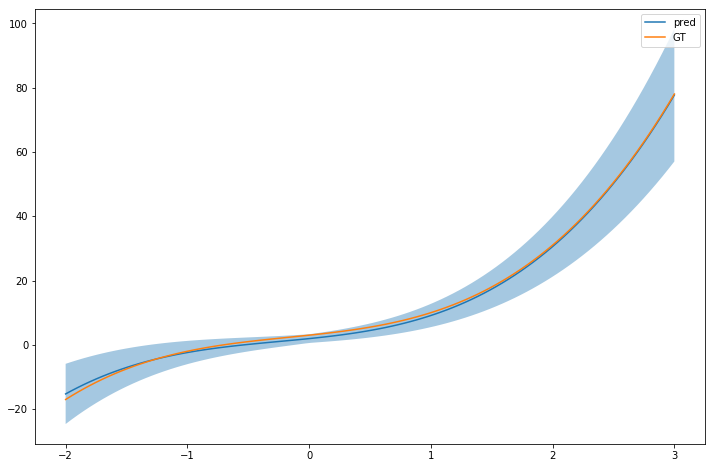
\includegraphics[width=200pt]{images/ex_3_2_a.png}
 \caption{True function, predicted function, with 95\% confidence band (pointwise).}
\end{figure}

\begin{figure}[ht]
 \centering
  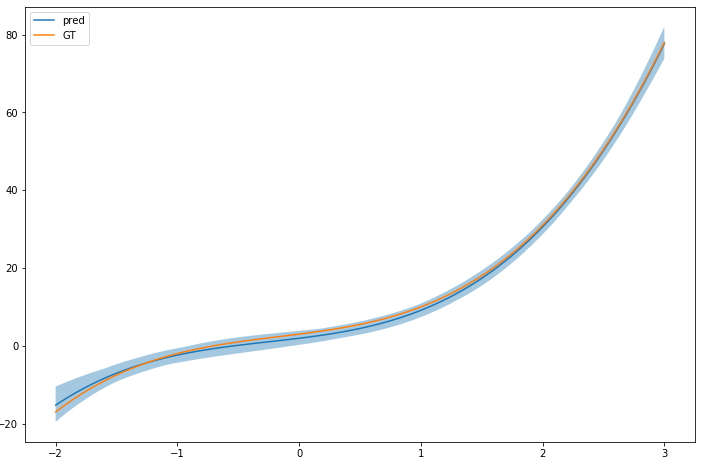
\includegraphics[width=200pt]{images/ex_3_2_b.png}
 \caption{True function, predicted function, with 95\% confidence band (from multivariate normal).}
\end{figure}

\subsubsection{Ex. 3.3}

\paragraph{a.} We formulate an estimate of $a^T\beta$ as $c^Ty$. For the least squares estimate we have that

\begin{equation}
    a^T \hat{\beta} = a^T (X^TX)^{-1}X^T y
\end{equation}

From this,

\begin{equation}
    c_0 = X(X^TX)^{-1}a
\end{equation}

Any $c$ can be written as

\begin{equation}
    c = c_0 + c_1 = X(X^TX)^{-1}a + c_1
\end{equation}

The constraint is that $\text{E}(c^Ty) = a^T\beta$.

\begin{equation}
    \text{E}(c^Ty) = \text{E}(c^T_0 y) + \text{E}(c^T_1 y) = a^T \beta
\end{equation}

Since $\text{E}(c^T_0 y) = a^T \beta$, we have that $\text{E}(c^T_1 \beta) = 0$.

\begin{equation}
    0 = \text{E}(c^T_1 y) = c^T_1 X \beta
\end{equation}

Because $\beta$ is unobservable, we conclude that

\begin{equation}
    0 = c^T_1 X
\end{equation}

which means

\begin{equation} \label{eq:ex3_3_a_constrain}
    c^T_1 c_0 = c^T_1 X (X^TX)^{-1}a = 0
\end{equation}

Now consider the variances.

\begin{equation}
    \text{Var}(a^T \hat{\beta}) = a^T \text{Var}(\hat{\beta}) a = \sigma^2 a^T (X^TX)^{-1} a
\end{equation}

Calculating the variance of a general unbiased estimate, using (\ref{eq:ex3_3_a_constrain}):

\begin{equation}
\begin{split}
    \text{Var}(c^T y) =& \sigma^2 c^T c\\
    =& \sigma^2 (c^T_0 + c^T_1)(c_0 + c_1) = \sigma^2 (c^T_0 c_0 + 0 + 0 + c^T_1 c_1)\\
    =& \sigma^2 c^T_0 c_0 + \sigma^2 c^T_1 c_1\\
    =& \text{Var}(a^T \hat{\beta}) + \sigma^2 c^T_1 c_1
\end{split}
\end{equation}

Since $\sigma^2 c^T_1 c_1 \ge 0$, we conclude that

\begin{equation}
    \text{Var}(c^Ty) \ge \text{Var}(a^T\hat{\beta})
\end{equation}

\paragraph{b.} The solution is basically the same as for the previous one. Here we will use the fact that $A^TA$ is a positive semidefinite matrix for any matrix $A$. A linear unbiased estimate for $\beta$ can be expressed as $\widetilde{\beta} = C^T y$, where $C$ is a $N \times (p+1)$ matrix. We can express $C$ as $C = X(X^TX)^{-1} + C_1 = C_0 + C_1$. The estimates are unbiased, so $\text{E}(C^Ty) = \beta$. From this we have

\begin{equation}
    \text{E}(C^Ty) = (C_0 + C_1)^T (X\beta) = \beta + C^T_1 X \beta = \beta \to C^T_1 X \beta = 0
\end{equation}

Because $\beta$ is unobservable, we have that

\begin{equation} \label{eq:ex3_3_b_constrain}
    C^T_1 X = 0
\end{equation}

Now consider the variances. $\hat{V} \equiv \text{Var}(\hat{\beta}) = \sigma^2 (X^TX)^{-1}$. $\tilde{V} \equiv \text{Var}(\tilde{\beta}) = \text{Var}(C^Ty) = \sigma^2 C^TC = \sigma^2 (C_0 + C_1)^T (C_0 + C_1)$. Using (\ref{eq:ex3_3_b_constrain}), we can write that $\tilde{V} = \sigma^2 C^T_0 C_0 + \sigma^2 C^T_1 C_1 = \hat{V} + \sigma^2 C^T_1 C_1$. From this: $\tilde{V} - \hat{V} = \sigma^2 C^T_1 C_1$ which is a positive semidefinite matrix. This concludes the proof.

\subsubsection{Ex. 3.5}

The ridge regression loss in vectorized form:

\[
L_{\text{ridge}} = (\mathbf{y} - \beta_0 \mathbf{e} - \mathbf{X}\bm{\beta})^T (\mathbf{y} - \beta_0 \mathbf{e} - \mathbf{X}\bm{\beta}) + \lambda \bm{\beta}^T\bm{\beta}
\]

$\mathbf{e}$ is a vector of all ones in $\mathbb{R}^N$. $\mathbf{X}$ is $N\times p$ matrix, so it doesn't have $\mathbf{e}$ as its first column. That's why we have a separate $\beta_0$, which is a scalar. All other coefficients are in the vector $\bm{\beta}$.

How to formulate $L^c_{\text{ridge}}$? We can use $L_{\text{ridge}}$, but instead of $\mathbf{X}$, we write $\mathbf{X} - \frac{1}{N}\mathbf{e}\mathbf{e}^T\mathbf{X}$. It's because $\frac{1}{N}\mathbf{e}^T\mathbf{X} = [\overline{x}_1, \overline{x}_2, \dots, \overline{x}_p]$. Let's create the following notation:

\[
    \mathbf{A} \equiv \frac{\mathbf{e}\mathbf{e}^T}{\mathbf{e}^T\mathbf{e}} = \frac{\mathbf{e}\mathbf{e}^T}{N}
\]

This is a projection onto the line defined by $\mathbf{e}$. So to get $L^c_{\text{ridge}}$, we replace $\mathbf{X}$ in $L_{\text{ridge}}$ with $(\mathbf{I} - \mathbf{A})\mathbf{X}$. So we only need to solve $L_{\text{ridge}}$ for $\beta_0$ and $\bm{\beta}$. Once we have these, we get $\beta^c_0$, $\bm{\beta}^c$ by applying the change $\mathbf{X} \to (\mathbf{I} - \mathbf{A})\mathbf{X}$.

\[
\begin{split}
\frac{\partial L_{\text{ridge}}}{\partial \beta_0} =& -2\mathbf{e}^T(\mathbf{y} - \beta_0 \mathbf{e} - \mathbf{X}\bm{\beta}) = 0\\
\to & \beta_0 = \overline{y} - \frac{1}{N}\mathbf{e}^T \mathbf{X} \bm{\beta}
\end{split}
\]

Note that $\mathbf{e}^T\mathbf{e} = N$, and $\mathbf{e}^T \mathbf{y} = N \overline{y}$. Now we can get $\beta^c_0$ by the above mentioned substitution. Note that $\mathbf{e}^T\mathbf{A} = \frac1N \mathbf{e}^T\mathbf{e}\mathbf{e}^T = \frac1N N\mathbf{e}^T = \mathbf{e}^T$.

\[
\begin{split}
\beta^c_0 =& \overline{y} - \frac1N \mathbf{e}^T (\mathbf{I} - \mathbf{A})\mathbf{X}\bm{\beta^c}\\
=& \overline{y} - \frac1N (\mathbf{e}^T\mathbf{I} - \mathbf{e}^T\mathbf{A})\mathbf{X}\bm{\beta^c}\\
=& \overline{y} - \frac1N (\mathbf{e}^T - \mathbf{e}^T)\mathbf{X}\bm{\beta^c}\\
=& \overline{y}
\end{split}
\]

So we see that $\beta^c_0$ does not depend on the features and coefficients, as $\beta_0$ does. Now let's move on to $\bm{\beta}$ and $\bm{\beta}^c$.

\[
\frac{\partial L_{\text{ridge}}}{\partial \bm{\beta}} = -2\mathbf{X}^T (\mathbf{y} - \beta_0 \mathbf{e} - \mathbf{X}\bm{\beta}) + 2\lambda \bm{\beta}
\]

Note that

\[
\beta_0 \mathbf{e} = \mathbf{e} \overline{y} - \frac1N \mathbf{e} \mathbf{e}^T \mathbf{X} \bm{\beta} = \mathbf{A}\mathbf{y} - \mathbf{A}\mathbf{X}\bm{\beta}
\]

So we have that

\[
\begin{split}
\frac{\partial L_{\text{ridge}}}{\partial \bm{\beta}} =& -2\mathbf{X}^T (\mathbf{y} - \mathbf{A}\mathbf{y} + \mathbf{A}\mathbf{X}\bm{\beta} - \mathbf{X}\bm{\beta}) + 2\lambda \bm{\beta} = 0\\
\to& \bm{\beta} = (\mathbf{X}^T(\mathbf{I} - \mathbf{A})\mathbf{X} + \lambda \mathbf{I})^{-1} \mathbf{X}^T (\mathbf{I} - \mathbf{A})\mathbf{y}
\end{split}
\]

From this we can get $\bm{\beta}^c$ (by the substitution $\mathbf{X} \to (\mathbf{I} - \mathbf{A})\mathbf{X}$). Note that $\mathbf{I} - \mathbf{A}$ is a projection, so its square is itself, as well as its transpose.

\[
\begin{split}
\bm{\beta}^c =& (((\mathbf{I} - \mathbf{A})\mathbf{X})^T(\mathbf{I} - \mathbf{A})(\mathbf{I} - \mathbf{A})\mathbf{X} + \lambda \mathbf{I})^{-1} ((\mathbf{I} - \mathbf{A})\mathbf{X})^T (\mathbf{I} - \mathbf{A})\mathbf{y}\\
=& (\mathbf{X}^T(\mathbf{I} - \mathbf{A})(\mathbf{I} - \mathbf{A})(\mathbf{I} - \mathbf{A})\mathbf{X} + \lambda \mathbf{I})^{-1} \mathbf{X}^T (\mathbf{I} - \mathbf{A})(\mathbf{I} - \mathbf{A})\mathbf{y}\\
=& (\mathbf{X}^T(\mathbf{I} - \mathbf{A})\mathbf{X} + \lambda \mathbf{I})^{-1} \mathbf{X}^T (\mathbf{I} - \mathbf{A})\mathbf{y}\\
=& \bm{\beta}
\end{split}
\]

So the conclusion is that by centering the inputs, we get the same result for $\bm{\beta}$ and $\bm{\beta}^c$, while $\beta_0$ gets replaces by $\beta^c_0 = \overline{y}$.

\subsubsection{Ex. 3.6}

\begin{itemize}
    \item $\bm{Y} = \bm{X}\bm{\beta} + \bm{\epsilon}$
    \item $\bm{\beta} \sim N(\bm{0}, \tau^2 \bm{I}_p)$
    \item $\bm{\epsilon} \sim N(\bm{0}, \sigma^2 \bm{I}_N)$
\end{itemize}

Using Appendix (\ref{app:Gaussian_posterior2}), $U=\beta$, $V=\bm{\epsilon}$, $W=XU+V=\bm{Y}$, we have that the posterior distribution $\beta | Y$ is Gaussian, with mean:

\[
\bm{\mu}_{\beta|y} = \tau^2 \bm{X}^T (\sigma^2 \bm{I}_N + \tau^2 \bm{X} \bm{X}^T)^{-1}\bm{y}
\]

Using the matrix inversion lemma described in Appendix (\ref{app:matrix_inv_lemma}), we can write that

\[
\begin{split}
(\tau^2\bm{X}\bm{X}^T + \sigma^2 \bm{I}_N)^{-1} = \frac{1}{\sigma^2}\left(\frac{\tau^2}{\sigma^2}\bm{X}\bm{X}^T + \bm{I}_N\right)^{-1}\\ =\frac{1}{\sigma^2}\left( \bm{I}_N - \frac{\tau}{\sigma} \bm{X}\left(\bm{I}_p + \frac{\tau^2}{\sigma^2}\bm{X}^T\bm{X}\right)^{-1}\frac{\tau}{\sigma}\bm{X}^T \right)\\
=\frac{1}{\sigma^2} \bm{I}_N - \frac{1}{\sigma^2} \bm{X}\left(\frac{\sigma^2}{\tau^2}\bm{I}_p + \bm{X}^T\bm{X}\right)^{-1}\bm{X}^T
\end{split}
\]

So the mean is:

\[
\begin{split}
\bm{\mu}_{\beta|y} =& \tau^2 \bm{X}^T (\sigma^2 \bm{I}_N + \tau^2 \bm{X} \bm{X}^T)^{-1}\bm{y}\\
=& \frac{\tau^2}{\sigma^2} \bm{X}^T\bm{y} - \frac{\tau^2}{\sigma^2}\bm{X}^T \bm{X}\left(\frac{\sigma^2}{\tau^2}\bm{I}_p + \bm{X}^T\bm{X}\right)^{-1}\bm{X}^T\bm{y}\\
=& \left[\frac{\tau^2}{\sigma^2} \left(\frac{\sigma^2}{\tau^2}\bm{I}_p + \bm{X}^T\bm{X}\right) - \frac{\tau^2}{\sigma^2}\bm{X}^T \bm{X}\right]\left(\frac{\sigma^2}{\tau^2}\bm{I}_p + \bm{X}^T\bm{X}\right)^{-1}\bm{X}^T\bm{y}\\
=& \left(\frac{\sigma^2}{\tau^2}\bm{I}_p + \bm{X}^T\bm{X}\right)^{-1}\bm{X}^T\bm{y}
\end{split}
\]

So this is the mean (and mode, as it is normally distributed) of $\beta$, given $\mathbf{y}$. We got the same expression as the one for ridge regression, when we have

\[
\lambda = \frac{\sigma^2}{\tau^2}
\]


\subsubsection{Ex. 3.8}

I assume that $\bm{X}$ has full rank, i.e., $\text{rank}(\bm{X}) = p+1$. We can write that $\bm{X} = [\bm{e} | \bm{X}_2]$, where $\bm{e}$ is the vector with all ones, and $\bm{X}_2$ is $N\times p$ matrix. Denote the column space of $\bm{X}$ by $W$, the subspace spanned by $\bm{e}$ is $W_e$, and so

\[
W = W_e + W_e^{\perp}
\]

By centering $\bm{X}_2$, we remove the projections of its columns onto $\bm{e}$, and so those columns will span $W_e^{\perp}$. the projection onto the line spanned by $\bm{e}$ is

\[
\bm{P}_e = \frac1N \bm{e}\bm{e}^T
\]

With this we have that

\[
\tilde{\bm{X}} = (\bm{I} - \bm{P}_e) \bm{X}_2
\]

because this way the columns of $\tilde{\bm{X}}$ are centered. The column space of $\tilde{\bm{X}}$ is $W_e^{\perp}$.

Considering the QR decomposition of $\bm{X}$, we can write:

\[
\bm{Q} = [\bm{e}/\sqrt{N} | \bm{Q}_2] = \frac{1}{\sqrt{N}} [\bm{e} | \sqrt{N} \bm{Q}_2]
\]

The SVD of $\tilde{\bm{X}}$:

\[
\tilde{\bm{X}} = \bm{U} \bm{D} \bm{V}^{T}
\]

Denote the column space of (arbitrary) $\bm{A}$ by $R(\bm{A})$. Then

\[
R(\tilde{\bm{X}}) = R(\bm{U}) = W_e^{\perp}
\]

\[
R(\bm{Q}_2) = W_e^{\perp}
\]


\subsubsection{Ex. 3.9 \emph{Forward stepwise regression}}

Actually we don't need $\mathbf{Q}$, we only need $\mathbf{H}= \mathbf{Q}\mathbf{Q}^T$, and updating this matrix. Some notations first. $W_1$ is the column space of $\mathbf{X}_1$. $\mathbf{u}$ is an arbitrary column vector of $\mathbf{X}_2$. $\mathbf{X}_{1u}$ is the matrix $[\mathbf{X_1} | \mathbf{u}]$. $W_{1u}$ is the column space of $\mathbf{X}_{1u}$. $\mathbf{H}_1$ is the projection matrix that projects onto $W_1$. $\mathbf{H}_{1u}$ projects onto $W_{1u}$.

We know the residual:

\[
\mathbf{r} = \mathbf{y} - \mathbf{\hat{y}} = \mathbf{y} - \mathbf{H}_1 \mathbf{y}
\]

Now the new residual:

\[
\mathbf{r}'  = \mathbf{y} - \mathbf{\hat{y}}' = \mathbf{y} - \mathbf{H}_{1u}\mathbf{y}
\]

Let's calculate $\mathbf{H}_{1u}$ efficiently. It projects onto $W_{1u}$. We have an orthonormal base in $W_1$, namely, the columns of $\mathbf{Q}$. We need an orthonormal base in $W_{1u}$ as well. So lets regress $\mathbf{u}$ onto $W_1$. $\mathbf{u}_p = \mathbf{H}_1 \mathbf{u}$ is the projection of $\mathbf{u}$ onto $W_1$, so $\mathbf{u} - \mathbf{H}_1 \mathbf{u}$ is orthogonal to $W_1$. Let's normalize this vector and append it to $\mathbf{Q}$.

\[
    \mathbf{q} = \frac{\mathbf{u} - \mathbf{H}_1 \mathbf{u}}{|| \mathbf{u} - \mathbf{H}_1 \mathbf{u} ||}
\]

With this we can construct $\mathbf{Q}' = [\mathbf{Q} | \mathbf{q}]$, and the columns of this matrix are orthonormal. The projection matrix:

\[
\mathbf{H}_{1u} = \mathbf{Q}'\mathbf{Q}'^T = \mathbf{Q}\mathbf{Q}^T + \mathbf{q}\mathbf{q}^T = \mathbf{H}_1 + \mathbf{q}\mathbf{q}^T
\]

The new residual:

\[
\mathbf{r}' = \mathbf{y} - \mathbf{H}_{1u}\mathbf{y} = \mathbf{y} - \mathbf{H}_1 \mathbf{y} - \mathbf{q}\mathbf{q}^T\mathbf{y} = \mathbf{r} - \mathbf{q}\mathbf{q}^T\mathbf{y}
\]

From this:

\[
\text{RSS}' = \text{RSS} -2\mathbf{r}^T \mathbf{q}\mathbf{q}^T \mathbf{y} + \mathbf{y}^T\mathbf{q}\mathbf{q}^T\mathbf{y}
\]

The drop in RSS:

\[
\text{RSS} - \text{RSS}' = (2\mathbf{r} - \mathbf{y})^T\mathbf{q}\mathbf{q}^T\mathbf{y}
\]

So we iterate through the columns of $\mathbf{X}_2$ and seek for the largest drop in RSS. Once we have the best column ($\mathbf{u}^{*}$), we pass $\mathbf{H}_{1u*}$ to the next iteration. Consider the notebook "forward\_stepwise.ipynb" where I have implemented this algorithm.

\subsubsection{Ex. 3.10 Backward stepwise regression}

Now we seek for a column vector $\mathbf{x}$ that we can drop from $\mathbf{X}$. Notations. $\mathbf{x}_i$ is the $i$th column vector of $\mathbf{X}$. $\mathbf{X}_i$ is the matrix obtained from $\mathbf{X}$ by dropping the $i$th column. $\mathbf{B} \equiv (\mathbf{X}^T\mathbf{X})^{-1}$. The $i$th column vector of $\mathbf{B}$ is $\mathbf{b}_i$.

Now, $\mathbf{H} = \mathbf{X}\mathbf{B}\mathbf{X}^T$ projects onto the column space of $\mathbf{X}$. According to Appendix (\ref{app:spec_Xb}), $\mathbf{H}_i = \mathbf{H} - \mathbf{P}_i$ projects onto the column space of $\mathbf{X}_i$, where

\[
\mathbf{P}_i = \frac{\mathbf{X}\mathbf{b}_i \mathbf{b}^T_i \mathbf{X}^T}{v_i}
\]

and $v_i$ is the $i$th element in the diagonal of $\mathbf{B}$. The original residual:

\[
\mathbf{r} = (\mathbf{I} - \mathbf{H})\mathbf{y}
\]

The new residual (after dropping the $i$th column in $\mathbf{X}$:

\[
\mathbf{r}_i = (\mathbf{I} - \mathbf{H}_i)\mathbf{y} = \mathbf{r} + \mathbf{P}_i \mathbf{y}
\]

From this we get the increment in RSS introduced by dropping the feature:

\[
\Delta \text{RSS}_i = (2\mathbf{r} + \mathbf{y})^T \mathbf{P}_i \mathbf{y}
\]

We seek for a column vector of $\mathbf{X}$ for which $\Delta\text{RSS}_i$ is minimal. We drop that feature. Consider the notebook "backward\_stepwise.ipynb" where I implement this algorithm.

\subsubsection{Ex. 3.11}

\[
\begin{split}
\text{RSS}(\mathbf{B}) =& \sum_{i=1}^{N} (y_i -f(x_i))^T \mathbf{\Sigma}^{-1} (y_i - f(x_i))\\
=& \text{Tr}\left( (\mathbf{Y} - \mathbf{X} \mathbf{B}) \mathbf{\Sigma}^{-1} (\mathbf{Y} - \mathbf{X} \mathbf{B})^T \right)\\
=&\text{Tr}(\mathbf{Y} \mathbf{\Sigma}^{-1} \mathbf{Y}^T) - \text{Tr}(\mathbf{Y} \mathbf{\Sigma}^{-1} \mathbf{B}^T \mathbf{X}^T) - \text{Tr}(\mathbf{X}\mathbf{B}\mathbf{\Sigma}^{-1}\mathbf{Y}^T) + \text{Tr}(\mathbf{X} \mathbf{B} \mathbf{\Sigma}^{-1} \mathbf{B}^T \mathbf{X}^T)
\end{split}
\]

Calculating the derivatives:

\[
\frac{d}{d\mathbf{B}}\text{Tr}(\mathbf{Y} \mathbf{\Sigma}^{-1} \mathbf{Y}^T) = \mathbf{0}
\]

\[
\frac{d}{d\mathbf{B}}\text{Tr}(\mathbf{Y} \mathbf{\Sigma}^{-1} \mathbf{B}^T \mathbf{X}^T) = \frac{d}{d\mathbf{B}}\text{Tr}(\mathbf{X}^T \mathbf{Y} \mathbf{\Sigma}^{-1} \mathbf{B}^T) = \mathbf{X}^T \mathbf{Y} \mathbf{\Sigma}^{-1}
\]

\[
\frac{d}{d\mathbf{B}}\text{Tr}(\mathbf{X}\mathbf{B}\mathbf{\Sigma}^{-1}\mathbf{Y}^T) = \frac{d}{d\mathbf{B}}\text{Tr}(\mathbf{\Sigma}^{-1}\mathbf{Y}^T\mathbf{X}\mathbf{B}) = (\mathbf{\Sigma}^{-1}\mathbf{Y}^T\mathbf{X})^T = \mathbf{X}^T \mathbf{Y} \mathbf{\Sigma}^{-1}
\]

\[
\begin{split}
\frac{d}{d\mathbf{B}}\text{Tr}(\mathbf{X} \mathbf{B} \mathbf{\Sigma}^{-1} \mathbf{B}^T \mathbf{X}^T) =& \frac{d}{d\mathbf{A}}\text{Tr}(\mathbf{X} \mathbf{A} \mathbf{\Sigma}^{-1} \mathbf{B}^T \mathbf{X}^T) + \frac{d}{d\mathbf{A}}\text{Tr}(\mathbf{X} \mathbf{B} \mathbf{\Sigma}^{-1} \mathbf{A}^T \mathbf{X}^T)\\
=& (\mathbf{\Sigma}^{-1} \mathbf{B}^T \mathbf{X}^T \mathbf{X})^T + \mathbf{X}^T \mathbf{X} \mathbf{B} \mathbf{\Sigma}^{-1}\\
=& 2\mathbf{X}^T \mathbf{X} \mathbf{B} \mathbf{\Sigma}^{-1}
\end{split}
\]

Now we can substitute:

\[
\frac{d}{d\mathbf{B}} \text{RSS}(\mathbf{B}) = -2 \mathbf{X}^T \mathbf{Y} \mathbf{\Sigma}^{-1} + 2\mathbf{X}^T \mathbf{X} \mathbf{B} \mathbf{\Sigma}^{-1}
\]

Setting this to zero, we get:

\[
\mathbf{B} = (\mathbf{X}^T\mathbf{X})^{-1}\mathbf{X}^T\mathbf{Y}
\]

What happens if the covariance matrices $\mathbf{\Sigma_i}$ are different for each observation? The Residual Sum of Squares:

\[
\text{RSS}(\mathbf{B}) = \sum_{i=1}^{N} (y_i - \mathbf{B}^Tx_i)^T \mathbf{\Sigma}^{-1}_i (y_i - \mathbf{B}^Tx_i)
\]

Derivating this w.r.t $\mathbf{B}$, and setting to zero, we get:

\[
\sum_{i=1}^{N} x_i x^T_i \mathbf{B} \mathbf{\Sigma}^{-1}_i = \sum_{i=1}^{N} x_i y^T_i \mathbf{\Sigma}^{-1}_i
\]

\subsubsection{Ex. 3.13}

Using the singular value decomposition of $X$,

\[
X = UDV^T
\]

the least squares coefficient is

\[
\begin{split}
\hat{\beta}^{ls} =& (X^TX)^{-1}X^Ty\\
=& (VDU^T UDV^T)^{-1}VDU^Ty\\
=& VD^{-2}V^T VDU^Ty=VD^{-1}U^Ty
\end{split}
\]

The PCR coefficient:

\[
\begin{split}
    \hat{\beta}^{pcr}(p) =& \sum_{m=1}^p \hat{\Theta}_m v_m = \sum_{m=1}^p \frac{z^T_m y}{z^T_m z_m} v_m\\
    =& \sum_{m=1}^p \frac{d_m u^T_m y}{d^2_m} v_m =\sum_{m=1}^p \frac{v_mu^T_m}{d_m} y = VD^{-1}U^T y
\end{split}
\]

which concludes the proof.


\newpage
\begin{appendices}

Here I collected the useful mathematical knowledge required to understand some proofs.

\section{differentiation}

\subsection{differentiation w.r.t. a vector}

\paragraph{1.} Let $\mathbf{a} \in \mathbb{R}^n$ be a constant vector, $\mathbf{x} \in \mathbb{R}^n$. Then

\begin{equation} \label{eq:da_dx}
    \frac{d}{d\mathbf{x}} (\mathbf{x}^{T}\mathbf{a}) = \frac{d}{d\mathbf{x}} (\mathbf{a}^{T}\mathbf{x}) = \mathbf{a}
\end{equation}

\paragraph{2.} Let $\mathbf{A} \in \mathbb{R}^{nxn}$ be a constant matrix, $\mathbf{x} \in \mathbb{R}^n$ Then

\begin{equation} \label{eq:dA_dx}
    \frac{d}{d\mathbf{x}} (\mathbf{x}^{T}\mathbf{A}\mathbf{x}) = (\mathbf{A} + \mathbf{A}^T) \mathbf{x}
\end{equation}

We can derive this as follows:

\[
\begin{split}
    \frac{d}{d\mathbf{x}} (\mathbf{x}^{T}\mathbf{A}\mathbf{x}) =& \frac{d}{d\mathbf{y}} (\mathbf{y}^{T}\mathbf{A}\mathbf{x}) + \frac{d}{d\mathbf{y}} (\mathbf{x}^{T}\mathbf{A}\mathbf{y})\\
    =& \frac{d}{d\mathbf{y}} (\mathbf{y}^{T}\mathbf{A}\mathbf{x}) + \frac{d}{d\mathbf{y}} (\mathbf{y}^T\mathbf{A}^{T}\mathbf{x})\\
    =& \mathbf{A}\mathbf{x} + \mathbf{A}^T\mathbf{x}
\end{split}
\]


\subsection{differentiation w.r.t. a matrix}

\paragraph{1.} Let $\mathbf{A} \in \mathbb{R}^{n\times m}$, $\mathbf{X} \in \mathbb{R}^{m\times n}$. Then

\begin{equation}
    \frac{d}{d\mathbf{X}}\text{Tr}(\mathbf{AX}) = \frac{d}{d\mathbf{X}}\text{Tr}(\mathbf{XA}) = \mathbf{A}^T
\end{equation}

\paragraph{2.} Let $\mathbf{A} \in \mathbb{R}^{n\times m}$, $\mathbf{X} \in \mathbb{R}^{n\times m}$. Then

\begin{equation}
    \frac{d}{d\mathbf{X}}\text{Tr}(\mathbf{AX^T}) = \frac{d}{d\mathbf{X}}\text{Tr}(\mathbf{X^TA}) = \mathbf{A}
\end{equation}


\paragraph{3.} Let $\mathbf{A} \in \mathbb{R}^{m\times m}$, $\mathbf{X} \in \mathbb{R}^{m\times n}$. Then

\begin{equation}
    \frac{d}{d\mathbf{X}} \text{Tr}(\mathbf{X}^T \mathbf{A} \mathbf{X}) = (\mathbf{A} + \mathbf{A}^T) \mathbf{X}
\end{equation}

We can derive it as follows:

\[
\begin{split}
    \frac{d}{d\mathbf{X}} \text{Tr}(\mathbf{X}^T \mathbf{A} \mathbf{X}) =& \frac{d}{d\mathbf{Y}} \text{Tr}(\mathbf{Y}^T \mathbf{A} \mathbf{X}) + \frac{d}{d\mathbf{Y}} \text{Tr}(\mathbf{X}^T \mathbf{A} \mathbf{Y})\\
    =& \mathbf{A} \mathbf{X} + (\mathbf{X}^T \mathbf{A})^T\\
    =& \mathbf{A} \mathbf{X} + \mathbf{A}^T \mathbf{X} = (\mathbf{A} + \mathbf{A}^T) \mathbf{X}
\end{split}
\]

\paragraph{Example.} Consider now this example.

\[
f(\mathbf{X}) = \text{Tr}(\mathbf{X}^T \mathbf{A} \mathbf{X} \mathbf{B} \mathbf{X}^T \mathbf{C})
\]

where $\mathbf{X} \in \mathbb{R}^{n\times m}$, $\mathbf{A} \in \mathbb{R}^{n\times n}$, $\mathbf{B} \in \mathbb{R}^{m\times m}$, $\mathbf{C} \in \mathbb{R}^{n\times m}$.

\[
\begin{split}
    \frac{d}{d\mathbf{X}} f(\mathbf{X}) =& \frac{d}{d\mathbf{Y}} \text{Tr}(\mathbf{Y}^T \mathbf{A} \mathbf{X} \mathbf{B} \mathbf{X}^T \mathbf{C})\\
    +& \frac{d}{d\mathbf{Y}} \text{Tr}(\mathbf{X}^T \mathbf{A} \mathbf{Y} \mathbf{B} \mathbf{X}^T \mathbf{C})\\
    +& \frac{d}{d\mathbf{Y}} \text{Tr}(\mathbf{X}^T \mathbf{A} \mathbf{X} \mathbf{B} \mathbf{Y}^T \mathbf{C})
\end{split}
\]

Calculating these:

\[
\begin{split}
    \frac{d}{d\mathbf{Y}} \text{Tr}(\mathbf{Y}^T \mathbf{A} \mathbf{X} \mathbf{B} \mathbf{X}^T \mathbf{C}) = \mathbf{A} \mathbf{X} \mathbf{B} \mathbf{X}^T \mathbf{C}
\end{split}
\]

\[
\begin{split}
    \frac{d}{d\mathbf{Y}} \text{Tr}(\mathbf{X}^T \mathbf{A} \mathbf{Y} \mathbf{B} \mathbf{X}^T \mathbf{C}) =& \frac{d}{d\mathbf{Y}} \text{Tr}(\mathbf{Y} \mathbf{B} \mathbf{X}^T \mathbf{C} \mathbf{X}^T \mathbf{A})\\
    =& (\mathbf{B} \mathbf{X}^T \mathbf{C} \mathbf{X}^T \mathbf{A})^T\\
    =& \mathbf{A}^T \mathbf{X} \mathbf{C}^T \mathbf{X} \mathbf{B}^T
\end{split}
\]

\[
\begin{split}
   \frac{d}{d\mathbf{Y}} \text{Tr}(\mathbf{X}^T \mathbf{A} \mathbf{X} \mathbf{B} \mathbf{Y}^T \mathbf{C}) = \frac{d}{d\mathbf{Y}} \text{Tr}(\mathbf{Y}^T \mathbf{C} \mathbf{X}^T \mathbf{A} \mathbf{X} \mathbf{B}) = \mathbf{C} \mathbf{X}^T \mathbf{A} \mathbf{X} \mathbf{B}
\end{split}
\]

So the result is:

\[
\frac{d}{d\mathbf{X}} \text{Tr}(\mathbf{X}^T \mathbf{A} \mathbf{X} \mathbf{B} \mathbf{X}^T \mathbf{C}) = \mathbf{A} \mathbf{X} \mathbf{B} \mathbf{X}^T \mathbf{C} + \mathbf{A}^T \mathbf{X} \mathbf{C}^T \mathbf{X} \mathbf{B}^T + \mathbf{C} \mathbf{X}^T \mathbf{A} \mathbf{X} \mathbf{B}
\]


\section{variance and covariance properties}

\subsection{scalar multiple}

We know that if $a \in \mathbb{R}$ is a constant scalar, and $X$ is a scalar random variable, then

\begin{equation}
    \text{Var}(aX) = a^2 \cdot \text{Var}(X)
\end{equation}

\subsection{vector multiple}

Now what if $a \in \mathbb{R}^{p}$ is a (constant) vector, and $X \in \mathbb{R}^{p}$ is a random vector, and we take the inner product $a^T\cdot X$? What is the variance $\text{Var}(a^T\cdot X)$?

\begin{flalign}
\begin{aligned}
    \text{Var}(a^T\cdot X) =& \text{Var}(a_1 \cdot X_1 + a_2 \cdot X_2 + \dots + a_n \cdot X_n)\\
    =& \text{E} \left( \sum_{i} a_i \cdot (X_i - \text{E} X_i)\right)^2\\
    =& \text{E} \left( \sum_{i,j} a_i  \cdot (X_i - \text{E} X_i) \cdot a_j \cdot (X_j - \text{E} X_j)\right)\\
    =& \sum_{i,j} a_i \cdot a_j \cdot \text{E} \left( (X_i - \text{E} X_i) \cdot (X_j - \text{E} X_j) \right)\\
    =& \sum_{i,j} a_i \cdot a_j \cdot \text{Cov}(X_i, X_j)\\
    =& a^T \cdot \text{Cov}(X,X) \cdot a = a^T \cdot \Sigma \cdot a
\end{aligned}
\end{flalign}

Here $\Sigma \equiv \text{Cov}(X,X)$ is the covariance matrix, $\text{Cov}(X,X)_{i,j} = \text{Cov}(X_i, X_j)$. Let's state our finding again. $a \in \mathbb{R}^{p}$ is a constant vector, $X \in \mathbb{R}^{p}$ is a random vector, then:

\begin{equation} \label{eq:vector_mul_variance}
    \text{Var}(a^T \cdot X) = a^T \cdot \text{Cov}(X,X) \cdot a
\end{equation}

Furthermore, we can write for the covariance matrix:

\begin{equation} \label{eq:covariance_formulae}
    \text{Cov}(X,X) = \text{E} ((X-\text{E}X)\cdot (X-\text{E}X)^T) = \text{E}(X\cdot X^T) - (\text{E}X) (\text{E}X^T)
\end{equation}

\subsection{matrix multiple}
Let $A \in \mathbb{R}^{nxp}$ a constant matrix, $X \in \mathbb{R}^{p}$ a random vector. The covariance matrix:

\begin{flalign} \label{eq:matrix_mul_cov}
\begin{aligned}
    \text{Cov}(AX) =& \text{E} (AXX^{T}A^{T}) - \text{E}(AX)\text{E}(X^{T}A^{T})\\
    =& A \cdot \text{E} (XX^{T}) \cdot A^{T} - A \cdot \text{E}(X) \text{E} (X^{T}) \cdot A^{T} \\
    =& A \cdot \left( \text{E} (XX^{T}) - \text{E}(X) \text{E}(X^{T}) \right) \cdot A^{T} \\
    =& A \cdot \text{Cov}(X) \cdot A^{T}
\end{aligned}
\end{flalign}

\section{distributions}

\subsection{Student's t-distribution}

The t-distribution with $\nu$ degrees of freedom can be expressed as

\begin{equation} \label{eq:t_distribution}
    T = \frac{Z}{\sqrt{V/\nu}}
\end{equation}

where

\begin{itemize}
    \item $Z\sim N(0,1)$
    \item $V\sim \chi_{\nu}^{2}$
    \item $Z$ and $V$ are independent
\end{itemize}

\subsection{F-distribution} \label{app:F_distribution}

A random variate of the F-distribution with parameters $d_1$ and $d_2$ arises as the ratio of two appropriately scaled chi-squared variates:

\begin{equation}
    X = \frac{U_1 / d_1}{U_2 / d_2}
\end{equation}

where

\begin{itemize}
    \item $U_{1}$ and $U_{2}$ have chi-squared distributions with $d_{1}$ and $d_{2}$ degrees of freedom respectively, and
    \item $U_{1}$ and $U_{2}$ are independent.
\end{itemize}

\subsection{Gaussian posterior distribution (W = U+V)} \label{app:Gaussian_posterior}

\begin{itemize}
    \item $U \sim N(\bm{\mu}_U \in \mathbb{R}^n, \bm{\Sigma}_U \in \mathbb{R}^{n\times n})$
    \item $V \sim N(\bm{\mu}_V \in \mathbb{R}^n, \bm{\Sigma}_V \in \mathbb{R}^{n\times n})$
    \item $U$ and $V$ are independent
\end{itemize}

$W = U + V$ is also normal, as well as $W|U$:

\begin{itemize}
    \item $W = U + V \sim N(\bm{\mu}_U + \bm{\mu}_V, \bm{\Sigma}_U + \bm{\Sigma}_V)$
    \item $W|U \sim N(U + \bm{\mu}_V, \bm{\Sigma}_V)$
\end{itemize}

The posterior distribution $U|W$ is Gaussian, this is what I want to prove here.

\begin{itemize}
    \item $U|W \sim N(\bm{\mu}_{U|W}, \bm{\Sigma}_{U|W})$
    \item $\bm{\mu}_{U|W} = \bm{\Sigma}_U (\bm{\Sigma}_U + \bm{\Sigma}_V)^{-1} (W - \bm{\mu}_V) + \bm{\Sigma}_V (\bm{\Sigma}_U + \bm{\Sigma}_V)^{-1}\bm{\mu}_U$
    \item $\bm{\Sigma}_{U|W} = \bm{\Sigma}_U (\bm{\Sigma}_U + \bm{\Sigma}_V)^{-1} \bm{\Sigma}_V = \bm{\Sigma}_V (\bm{\Sigma}_U + \bm{\Sigma}_V)^{-1} \bm{\Sigma}_U$
\end{itemize}

The proof is too long, I won't specify all the details here. First, assuming that both $U$ and $V$ have a pdf,

\[
f_{U|W}(u|w) = \frac{f_{W|U}(w|u) f_{U}(u)}{f_{W}(w)}
\]

where

\[
f_{W|U}(w|u) = \frac{\text{exp}\left(-\frac12 (w-u-\mu_V)^T \bm{\Sigma}_V^{-1} (w-u-\mu_V) \right)}{\sqrt{(2\pi)^n \text{det}(\bm{\Sigma}_V)}}
\]

\[
f_{U}(u) = \frac{\text{exp}\left( -\frac12 (u-\mu_U)^T \bm{\Sigma}^{-1}_U (u-\mu_U) \right)}{\sqrt{(2\pi)^n \text{det}(\bm{\Sigma}_U)}}
\]

\[
f_{W}(w) = \frac{\text{exp}\left( -\frac12 (w-\mu_U-\mu_V)^T (\bm{\Sigma}_U + \bm{\Sigma}_V)^{-1} (w-\mu_U-\mu_V) \right)}{\sqrt{(2\pi)^n \text{det}(\bm{\Sigma}_U + \bm{\Sigma}_V)}}
\]

Plugging these into the equation above, after a lot of computation, we get to

\[
f_{U|W}(u|w) = \frac{\text{exp}\left( -\frac12 (u-\mu_{U|W})^T \bm{\Sigma}_{U|W}^{-1} (u-\mu_{U|W}) \right)}{\sqrt{(2\pi)^n \text{det}(\bm{\Sigma}_{U|W})}}
\]



\subsection{Gaussian posterior distribution (W = XU+V)} \label{app:Gaussian_posterior2}

\begin{itemize}
    \item $U \sim N(\bm{\mu}_U \in \mathbb{R}^m, \bm{\Sigma}_U \in \mathbb{R}^{m\times m})$
    \item $V \sim N(\bm{\mu}_V \in \mathbb{R}^n, \bm{\Sigma}_V \in \mathbb{R}^{n\times n})$
    \item $U$ and $V$ are independent
    \item $X \in \mathbb{R}^{n\times m}$, non-random
\end{itemize}

$W = \bm{X}U + V$ is also normal, as well as $W|U$:

\begin{itemize}
    \item $W = \bm{X}U + V \sim N(\bm{X}\bm{\mu}_U + \bm{\mu}_V, \bm{X}\bm{\Sigma}_U\bm{X}^T + \bm{\Sigma}_V)$
    \item $W|U \sim N(\bm{X}U + \bm{\mu}_V, \bm{\Sigma}_V)$
\end{itemize}

The posterior distribution $U|W$ is Gaussian, but I don't prove it here.

\begin{itemize}
    \item $U|W \sim N(\bm{\mu}_{U|W}, \bm{\Sigma}_{U|W})$
    \item $\bm{\mu}_{U|W} = (\bm{I} - \bm{\Sigma}_U \bm{X}^T \bm{C}) \bm{\mu}_U + \bm{\Sigma}_U \bm{X}^T \bm{C}(W - \bm{\mu}_V)$
    \item $\bm{\Sigma}_{U|W} =\bm{\Sigma}_U - \bm{\Sigma}_U \bm{X}^T \bm{C} \bm{X} \bm{\Sigma}_U$
    \item $\bm{C} \equiv (\bm{\Sigma}_V + \bm{X} \bm{\Sigma}_U \bm{X}^T)^{-1}$
\end{itemize}



\section{projections}

\subsection{sum of projections}

Let $V$ be a vector space, $W_1 \subset V$ a subspace, $W_2 \subset V$ a subspace such that $W_1 \perp W_2$.

Let $P_1$ be an orthogonal projection onto the subspace $W_1$, $P_2$ be an orthogonal projection onto the subspace $W_2$. I claim that $P_1 + P_2$ is an orthogonal projection onto $W_1 + W_2$.

\begin{proof}

Denote $W_{\perp}$ the orthogonal complement of $W_1+W_2$.

\begin{equation}
    (W_1 + W_2) + W_{\perp} = V
\end{equation}

and

\begin{equation}
    (W_1 + W_2) \perp W_{\perp}
\end{equation}

Any vector $v \in V$ can be decomposed as

\begin{equation}
    v = w_{\perp} + w_1 + w_2
\end{equation}

where $w_{\perp} \in W_{\perp}$, $w_1 \in W_1$, $w_2 \in W_2$. This decomposition is unique.

\begin{equation}
    P_1 v = 0 + w_1 + 0 = w_1
\end{equation}

\begin{equation}
    P_2 v = 0 + 0 + w_2 = w_2
\end{equation}

From these

\begin{equation}
    (P_1 + P_2) v = w_1 + w_2
\end{equation}

So $P_1 + P_2$ projects onto $W_1 + W_2$.

\end{proof}


\subsection{difference of projections} \label{app:diff_proj}

Let $V$ be a vector space, $W_1 \subset V$ a subspace, $W_2 \subset W_1$ a subspace, $W_3 \subset W_1$ a subspace, such that $W_2 \perp W_3$, and $W_2 + W_3 = W_1$.

Let $P_1$ be an orthogonal projection onto the subspace $W_1$, $P_2$ be an orthogonal projection onto the subspace $W_2$. I claim that $P_1 - P_2$ is an orthogonal projection onto $W_3$.

\begin{proof}
Denote $W_{\perp}$ the orthogonal complement of $W_1$: $W_1 + W_{\perp} = V$, and $W_1 \perp W_{\perp}$

Any vector $v \in V$ can be decomposed as

\begin{equation}
    v = w_{\perp} + w_2 + w_3
\end{equation}

where $w_{\perp} \in W_{\perp}$, $w_2 \in W_2$, $w_3 \in W_3$. This decomposition is unique.

\begin{equation}
    P_1 v = 0 + w_2 + w_3 = w_2 + w_3
\end{equation}

\begin{equation}
    P_2 v = 0 + w_2 + 0 = w_2
\end{equation}

From these

\begin{equation}
    (P_1 - P_2) v = (w_2 + w_3) - w_2 = w_3
\end{equation}

So $P_1 - P_2$ projects onto $W_3$.

\end{proof}

\subsection{The special vector $Xb$} \label{app:spec_Xb}

(I couldn't find any better name for this subsection, sorry for this...) Let's begin with the $N\times p$ matrix $X$, where we denote the column vectors by $x_i$. Assume that $X$ has a full column-rank, so $\text{rank}(X)=p$. Denote the subspace $W = span(x_1, x_2, \dots, x_{p-1})$, which is the subspace generated by all the columns of $X$, except the last one. Let $b$ be the last column vector of $(X^TX)^{-1}$. I claim that $Xb$ is a vector that is perpendicular to $W$. Obviously, $Xb$ is in the column space of $X$. We have that

\begin{equation}
    X^TX(X^TX)^{-1} = I
\end{equation}

Considering the $i$th row, $j$th column ($q_j$ being the $j$th column vector of $(X^TX)^{-1}$, so $q_p = b$)

\begin{equation}
    x^T_i X q_j = \delta_{i,j}
\end{equation}

Choosing $j=p$

\begin{equation}
    x^T_i X b = \delta_{i,p}
\end{equation}

This means that $Xb$ is perpendicular to $x_i$ ($i \neq p$), which is what I wanted to prove. Now let's project onto the subspace $W_p = \text{span}(Xb)$:

\begin{equation}
    P_{p} = \frac{Xb\cdot b^TX^T}{b^TX^TXb} = \frac{Xb\cdot b^TX^T}{v}
\end{equation}

where $v \equiv b_p$ is the last element of the vector $b$, that is, $v\equiv [(X^TX)^{-1}]_{p,p}$.

Now we can create the same projection according to Appendix \ref{app:diff_proj}. Let $P_X$ be the projection onto the column space of $X$, and $P_W$ the projection onto $W$:

\begin{equation}
    P_X = X (X^TX)^{-1} X^T
\end{equation}

\begin{equation}
    P_W = X_0 (X^T_0 X_0)^{-1} X^T_0
\end{equation}

where we get $X_0$ from $X$ by dropping the last column. Now we see that

\begin{equation}
    X (X^TX)^{-1} X^T - X_0 (X^T_0 X_0)^{-1} X^T_0 = \frac{Xb\cdot b^TX^T}{v}
\end{equation}

\section{Matrices}

\subsection{The matrix inversion lemma}\label{app:matrix_inv_lemma}

A special form of the matrix inversion lemma:

\[
(\bm{I}_n + \bm{U}\bm{V})^{-1} = \bm{I}_n - \bm{U}(\bm{I}_m + \bm{V}\bm{U})^{-1}\bm{V}
\]

where $\bm{U} \in \mathbb{R}^{n\times m}$, $\bm{V} \in \mathbb{R}^{m\times n}$.

Proof.

\[
(\bm{I}_n + \bm{U}\bm{V})^{-1} = \bm{I}_n - (\bm{I}_n + \bm{U}\bm{V})^{-1}\bm{U}\bm{V} = \bm{I}_n - \bm{U}(\bm{I}_m + \bm{V}\bm{U})^{-1}\bm{V}
\]

At first we used the following:

\[
(\bm{I} + \bm{P})^{-1} = \bm{I} - (\bm{I} + \bm{P})^{-1} \bm{P}
\]

which comes from:

\[
\begin{split}
(\bm{I} + \bm{P})^{-1}(\bm{I} + \bm{P}) =& \bm{I}\\
(\bm{I} + \bm{P})^{-1} + (\bm{I} + \bm{P})^{-1} \bm{P} =& \bm{I}\\
(\bm{I} + \bm{P})^{-1} =& \bm{I} - (\bm{I} + \bm{P})^{-1} \bm{P}
\end{split}
\]

Secondly, we used:

\[
(\bm{I}_n+\bm{U}\bm{V})^{-1}\bm{U} = \bm{U}(\bm{I}_m+\bm{V}\bm{U})^{-1}
\]

which comes from:

\[
\begin{split}
    \bm{U}(\bm{I}_m + \bm{V}\bm{U}) = (\bm{I}_n + \bm{U}\bm{V})\bm{U}\\
    (\bm{I}_n + \bm{U}\bm{V})^{-1}\bm{U}(\bm{I}_m+\bm{V}\bm{U}) = \bm{U}\\
    (\bm{I}_n+\bm{U}\bm{V})^{-1}\bm{U} = \bm{U}(\bm{I}_m+\bm{V}\bm{U})^{-1}
\end{split}
\]

which concludes the proof.

\end{appendices}

\end{document}
